\documentclass[twoside]{book}

% Packages required by doxygen
\usepackage{fixltx2e}
\usepackage{calc}
\usepackage{doxygen}
\usepackage[export]{adjustbox} % also loads graphicx
\usepackage{graphicx}
\usepackage[utf8]{inputenc}
\usepackage{makeidx}
\usepackage{multicol}
\usepackage{multirow}
\PassOptionsToPackage{warn}{textcomp}
\usepackage{textcomp}
\usepackage[nointegrals]{wasysym}
\usepackage[table]{xcolor}

% Font selection
\usepackage[T1]{fontenc}
\usepackage[scaled=.90]{helvet}
\usepackage{courier}
\usepackage{amssymb}
\usepackage{sectsty}
\renewcommand{\familydefault}{\sfdefault}
\allsectionsfont{%
  \fontseries{bc}\selectfont%
  \color{darkgray}%
}
\renewcommand{\DoxyLabelFont}{%
  \fontseries{bc}\selectfont%
  \color{darkgray}%
}
\newcommand{\+}{\discretionary{\mbox{\scriptsize$\hookleftarrow$}}{}{}}

% Page & text layout
\usepackage{geometry}
\geometry{%
  a4paper,%
  top=2.5cm,%
  bottom=2.5cm,%
  left=2.5cm,%
  right=2.5cm%
}
\tolerance=750
\hfuzz=15pt
\hbadness=750
\setlength{\emergencystretch}{15pt}
\setlength{\parindent}{0cm}
\setlength{\parskip}{3ex plus 2ex minus 2ex}
\makeatletter
\renewcommand{\paragraph}{%
  \@startsection{paragraph}{4}{0ex}{-1.0ex}{1.0ex}{%
    \normalfont\normalsize\bfseries\SS@parafont%
  }%
}
\renewcommand{\subparagraph}{%
  \@startsection{subparagraph}{5}{0ex}{-1.0ex}{1.0ex}{%
    \normalfont\normalsize\bfseries\SS@subparafont%
  }%
}
\makeatother

% Headers & footers
\usepackage{fancyhdr}
\pagestyle{fancyplain}
\fancyhead[LE]{\fancyplain{}{\bfseries\thepage}}
\fancyhead[CE]{\fancyplain{}{}}
\fancyhead[RE]{\fancyplain{}{\bfseries\leftmark}}
\fancyhead[LO]{\fancyplain{}{\bfseries\rightmark}}
\fancyhead[CO]{\fancyplain{}{}}
\fancyhead[RO]{\fancyplain{}{\bfseries\thepage}}
\fancyfoot[LE]{\fancyplain{}{}}
\fancyfoot[CE]{\fancyplain{}{}}
\fancyfoot[RE]{\fancyplain{}{\bfseries\scriptsize Generated by Doxygen }}
\fancyfoot[LO]{\fancyplain{}{\bfseries\scriptsize Generated by Doxygen }}
\fancyfoot[CO]{\fancyplain{}{}}
\fancyfoot[RO]{\fancyplain{}{}}
\renewcommand{\footrulewidth}{0.4pt}
\renewcommand{\chaptermark}[1]{%
  \markboth{#1}{}%
}
\renewcommand{\sectionmark}[1]{%
  \markright{\thesection\ #1}%
}

% Indices & bibliography
\usepackage{natbib}
\usepackage[titles]{tocloft}
\setcounter{tocdepth}{3}
\setcounter{secnumdepth}{5}
\makeindex

% Hyperlinks (required, but should be loaded last)
\usepackage{ifpdf}
\ifpdf
  \usepackage[pdftex,pagebackref=true]{hyperref}
\else
  \usepackage[ps2pdf,pagebackref=true]{hyperref}
\fi
\hypersetup{%
  colorlinks=true,%
  linkcolor=blue,%
  citecolor=blue,%
  unicode%
}

% Custom commands
\newcommand{\clearemptydoublepage}{%
  \newpage{\pagestyle{empty}\cleardoublepage}%
}

\usepackage{caption}
\captionsetup{labelsep=space,justification=centering,font={bf},singlelinecheck=off,skip=4pt,position=top}

%===== C O N T E N T S =====

\begin{document}

% Titlepage & ToC
\hypersetup{pageanchor=false,
             bookmarksnumbered=true,
             pdfencoding=unicode
            }
\pagenumbering{alph}
\begin{titlepage}
\vspace*{7cm}
\begin{center}%
{\Large Rogue Two \\[1ex]\large 0.\+1 }\\
\vspace*{1cm}
{\large Generated by Doxygen 1.8.14}\\
\end{center}
\end{titlepage}
\clearemptydoublepage
\pagenumbering{roman}
\tableofcontents
\clearemptydoublepage
\pagenumbering{arabic}
\hypersetup{pageanchor=true}

%--- Begin generated contents ---
\chapter{Namespace Index}
\section{Packages}
Here are the packages with brief descriptions (if available)\+:\begin{DoxyCompactList}
\item\contentsline{section}{\mbox{\hyperlink{namespace_ecs}{Ecs}} }{\pageref{namespace_ecs}}{}
\item\contentsline{section}{\mbox{\hyperlink{namespace_game}{Game}} }{\pageref{namespace_game}}{}
\item\contentsline{section}{\mbox{\hyperlink{namespace_game_1_1_components}{Game.\+Components}} }{\pageref{namespace_game_1_1_components}}{}
\item\contentsline{section}{\mbox{\hyperlink{namespace_game_1_1_data}{Game.\+Data}} }{\pageref{namespace_game_1_1_data}}{}
\item\contentsline{section}{\mbox{\hyperlink{namespace_game_1_1_data_structures}{Game.\+Data\+Structures}} }{\pageref{namespace_game_1_1_data_structures}}{}
\item\contentsline{section}{\mbox{\hyperlink{namespace_game_1_1_dungeon_maker}{Game.\+Dungeon\+Maker}} }{\pageref{namespace_game_1_1_dungeon_maker}}{}
\item\contentsline{section}{\mbox{\hyperlink{namespace_game_1_1_interfaces}{Game.\+Interfaces}} }{\pageref{namespace_game_1_1_interfaces}}{}
\item\contentsline{section}{\mbox{\hyperlink{namespace_i_o}{IO}} }{\pageref{namespace_i_o}}{}
\end{DoxyCompactList}

\chapter{Hierarchical Index}
\section{Class Hierarchy}
This inheritance list is sorted roughly, but not completely, alphabetically\+:\begin{DoxyCompactList}
\item \contentsline{section}{Game.\+Application}{\pageref{class_game_1_1_application}}{}
\item \contentsline{section}{Game.\+Dungeon\+Maker.\+Basic\+Dungeon}{\pageref{class_game_1_1_dungeon_maker_1_1_basic_dungeon}}{}
\item \contentsline{section}{Game.\+Dungeon\+Maker.\+Cell}{\pageref{class_game_1_1_dungeon_maker_1_1_cell}}{}
\item \contentsline{section}{Ecs.\+Component}{\pageref{class_ecs_1_1_component}}{}
\begin{DoxyCompactList}
\item \contentsline{section}{Ecs.\+Transform}{\pageref{class_ecs_1_1_transform}}{}
\item \contentsline{section}{Game.\+Components.\+Actor}{\pageref{class_game_1_1_components_1_1_actor}}{}
\begin{DoxyCompactList}
\item \contentsline{section}{Game.\+Components.\+Enemy}{\pageref{class_game_1_1_components_1_1_enemy}}{}
\item \contentsline{section}{Game.\+Components.\+Player}{\pageref{class_game_1_1_components_1_1_player}}{}
\end{DoxyCompactList}
\item \contentsline{section}{Game.\+Components.\+Collider}{\pageref{class_game_1_1_components_1_1_collider}}{}
\item \contentsline{section}{Game.\+Components.\+Door}{\pageref{class_game_1_1_components_1_1_door}}{}
\item \contentsline{section}{Game.\+Components.\+Game\+Manager}{\pageref{class_game_1_1_components_1_1_game_manager}}{}
\item \contentsline{section}{Game.\+Components.\+H\+UD}{\pageref{class_game_1_1_components_1_1_h_u_d}}{}
\item \contentsline{section}{Game.\+Components.\+Map}{\pageref{class_game_1_1_components_1_1_map}}{}
\item \contentsline{section}{Game.\+Components.\+Model}{\pageref{class_game_1_1_components_1_1_model}}{}
\item \contentsline{section}{Game.\+Components.\+Player\+Controller}{\pageref{class_game_1_1_components_1_1_player_controller}}{}
\item \contentsline{section}{Game.\+Components.\+Sound}{\pageref{class_game_1_1_components_1_1_sound}}{}
\item \contentsline{section}{Game.\+Components.\+Spawn\+Manager}{\pageref{class_game_1_1_components_1_1_spawn_manager}}{}
\end{DoxyCompactList}
\item \contentsline{section}{I\+O.\+Console\+UI}{\pageref{class_i_o_1_1_console_u_i}}{}
\item \contentsline{section}{Game.\+Dungeon\+Maker.\+Coord}{\pageref{class_game_1_1_dungeon_maker_1_1_coord}}{}
\item \contentsline{section}{I\+O.\+Debug}{\pageref{class_i_o_1_1_debug}}{}
\item \contentsline{section}{Ecs.\+Game\+Object}{\pageref{class_ecs_1_1_game_object}}{}
\item \contentsline{section}{Game.\+Interfaces.\+I\+Damageable}{\pageref{interface_game_1_1_interfaces_1_1_i_damageable}}{}
\begin{DoxyCompactList}
\item \contentsline{section}{Game.\+Components.\+Enemy}{\pageref{class_game_1_1_components_1_1_enemy}}{}
\item \contentsline{section}{Game.\+Components.\+Player}{\pageref{class_game_1_1_components_1_1_player}}{}
\end{DoxyCompactList}
\item \contentsline{section}{Game.\+Interfaces.\+I\+Movable}{\pageref{interface_game_1_1_interfaces_1_1_i_movable}}{}
\begin{DoxyCompactList}
\item \contentsline{section}{Game.\+Components.\+Enemy}{\pageref{class_game_1_1_components_1_1_enemy}}{}
\item \contentsline{section}{Game.\+Components.\+Player}{\pageref{class_game_1_1_components_1_1_player}}{}
\item \contentsline{section}{Game.\+Components.\+Player\+Controller}{\pageref{class_game_1_1_components_1_1_player_controller}}{}
\item \contentsline{section}{Game.\+Components.\+Sound}{\pageref{class_game_1_1_components_1_1_sound}}{}
\end{DoxyCompactList}
\item \contentsline{section}{I\+O.\+Input}{\pageref{class_i_o_1_1_input}}{}
\item \contentsline{section}{Game.\+Data.\+Monster\+Generator}{\pageref{class_game_1_1_data_1_1_monster_generator}}{}
\item \contentsline{section}{Program}{\pageref{class_program}}{}
\item \contentsline{section}{Game.\+Dungeon\+Maker.\+Room}{\pageref{class_game_1_1_dungeon_maker_1_1_room}}{}
\item \contentsline{section}{Ecs.\+Time}{\pageref{class_ecs_1_1_time}}{}
\item \contentsline{section}{Ecs.\+Vec2i}{\pageref{class_ecs_1_1_vec2i}}{}
\end{DoxyCompactList}

\chapter{Class Index}
\section{Class List}
Here are the classes, structs, unions and interfaces with brief descriptions\+:\begin{DoxyCompactList}
\item\contentsline{section}{\mbox{\hyperlink{class_game_1_1_components_1_1_actor}{Game.\+Components.\+Actor}} }{\pageref{class_game_1_1_components_1_1_actor}}{}
\item\contentsline{section}{\mbox{\hyperlink{class_game_1_1_application}{Game.\+Application}} }{\pageref{class_game_1_1_application}}{}
\item\contentsline{section}{\mbox{\hyperlink{class_game_1_1_dungeon_maker_1_1_basic_dungeon}{Game.\+Dungeon\+Maker.\+Basic\+Dungeon}} }{\pageref{class_game_1_1_dungeon_maker_1_1_basic_dungeon}}{}
\item\contentsline{section}{\mbox{\hyperlink{class_game_1_1_dungeon_maker_1_1_cell}{Game.\+Dungeon\+Maker.\+Cell}} }{\pageref{class_game_1_1_dungeon_maker_1_1_cell}}{}
\item\contentsline{section}{\mbox{\hyperlink{class_game_1_1_components_1_1_collider}{Game.\+Components.\+Collider}} }{\pageref{class_game_1_1_components_1_1_collider}}{}
\item\contentsline{section}{\mbox{\hyperlink{class_ecs_1_1_component}{Ecs.\+Component}} }{\pageref{class_ecs_1_1_component}}{}
\item\contentsline{section}{\mbox{\hyperlink{class_i_o_1_1_console_u_i}{I\+O.\+Console\+UI}} }{\pageref{class_i_o_1_1_console_u_i}}{}
\item\contentsline{section}{\mbox{\hyperlink{class_game_1_1_dungeon_maker_1_1_coord}{Game.\+Dungeon\+Maker.\+Coord}} }{\pageref{class_game_1_1_dungeon_maker_1_1_coord}}{}
\item\contentsline{section}{\mbox{\hyperlink{class_i_o_1_1_debug}{I\+O.\+Debug}} }{\pageref{class_i_o_1_1_debug}}{}
\item\contentsline{section}{\mbox{\hyperlink{class_game_1_1_components_1_1_door}{Game.\+Components.\+Door}} }{\pageref{class_game_1_1_components_1_1_door}}{}
\item\contentsline{section}{\mbox{\hyperlink{class_game_1_1_components_1_1_enemy}{Game.\+Components.\+Enemy}} }{\pageref{class_game_1_1_components_1_1_enemy}}{}
\item\contentsline{section}{\mbox{\hyperlink{class_game_1_1_components_1_1_game_manager}{Game.\+Components.\+Game\+Manager}} }{\pageref{class_game_1_1_components_1_1_game_manager}}{}
\item\contentsline{section}{\mbox{\hyperlink{class_ecs_1_1_game_object}{Ecs.\+Game\+Object}} }{\pageref{class_ecs_1_1_game_object}}{}
\item\contentsline{section}{\mbox{\hyperlink{class_game_1_1_components_1_1_h_u_d}{Game.\+Components.\+H\+UD}} }{\pageref{class_game_1_1_components_1_1_h_u_d}}{}
\item\contentsline{section}{\mbox{\hyperlink{interface_game_1_1_interfaces_1_1_i_damageable}{Game.\+Interfaces.\+I\+Damageable}} }{\pageref{interface_game_1_1_interfaces_1_1_i_damageable}}{}
\item\contentsline{section}{\mbox{\hyperlink{interface_game_1_1_interfaces_1_1_i_movable}{Game.\+Interfaces.\+I\+Movable}} }{\pageref{interface_game_1_1_interfaces_1_1_i_movable}}{}
\item\contentsline{section}{\mbox{\hyperlink{class_i_o_1_1_input}{I\+O.\+Input}} }{\pageref{class_i_o_1_1_input}}{}
\item\contentsline{section}{\mbox{\hyperlink{class_game_1_1_components_1_1_map}{Game.\+Components.\+Map}} }{\pageref{class_game_1_1_components_1_1_map}}{}
\item\contentsline{section}{\mbox{\hyperlink{class_game_1_1_components_1_1_model}{Game.\+Components.\+Model}} }{\pageref{class_game_1_1_components_1_1_model}}{}
\item\contentsline{section}{\mbox{\hyperlink{class_game_1_1_data_1_1_monster_generator}{Game.\+Data.\+Monster\+Generator}} }{\pageref{class_game_1_1_data_1_1_monster_generator}}{}
\item\contentsline{section}{\mbox{\hyperlink{class_game_1_1_components_1_1_player}{Game.\+Components.\+Player}} }{\pageref{class_game_1_1_components_1_1_player}}{}
\item\contentsline{section}{\mbox{\hyperlink{class_game_1_1_components_1_1_player_controller}{Game.\+Components.\+Player\+Controller}} }{\pageref{class_game_1_1_components_1_1_player_controller}}{}
\item\contentsline{section}{\mbox{\hyperlink{class_program}{Program}} }{\pageref{class_program}}{}
\item\contentsline{section}{\mbox{\hyperlink{class_game_1_1_dungeon_maker_1_1_room}{Game.\+Dungeon\+Maker.\+Room}} }{\pageref{class_game_1_1_dungeon_maker_1_1_room}}{}
\item\contentsline{section}{\mbox{\hyperlink{class_game_1_1_components_1_1_sound}{Game.\+Components.\+Sound}} }{\pageref{class_game_1_1_components_1_1_sound}}{}
\item\contentsline{section}{\mbox{\hyperlink{class_game_1_1_components_1_1_spawn_manager}{Game.\+Components.\+Spawn\+Manager}} }{\pageref{class_game_1_1_components_1_1_spawn_manager}}{}
\item\contentsline{section}{\mbox{\hyperlink{class_ecs_1_1_time}{Ecs.\+Time}} }{\pageref{class_ecs_1_1_time}}{}
\item\contentsline{section}{\mbox{\hyperlink{class_ecs_1_1_transform}{Ecs.\+Transform}} }{\pageref{class_ecs_1_1_transform}}{}
\item\contentsline{section}{\mbox{\hyperlink{class_ecs_1_1_vec2i}{Ecs.\+Vec2i}} }{\pageref{class_ecs_1_1_vec2i}}{}
\end{DoxyCompactList}

\chapter{Namespace Documentation}
\hypertarget{namespace_ecs}{}\section{Ecs Namespace Reference}
\label{namespace_ecs}\index{Ecs@{Ecs}}
\subsection*{Classes}
\begin{DoxyCompactItemize}
\item 
class \mbox{\hyperlink{class_ecs_1_1_component}{Component}}
\item 
class \mbox{\hyperlink{class_ecs_1_1_game_object}{Game\+Object}}
\item 
class \mbox{\hyperlink{class_ecs_1_1_time}{Time}}
\item 
class \mbox{\hyperlink{class_ecs_1_1_transform}{Transform}}
\item 
class \mbox{\hyperlink{class_ecs_1_1_vec2i}{Vec2i}}
\end{DoxyCompactItemize}

\hypertarget{namespace_game}{}\section{Game Namespace Reference}
\label{namespace_game}\index{Game@{Game}}
\subsection*{Namespaces}
\begin{DoxyCompactItemize}
\end{DoxyCompactItemize}
\subsection*{Classes}
\begin{DoxyCompactItemize}
\item 
class \mbox{\hyperlink{class_game_1_1_application}{Application}}
\end{DoxyCompactItemize}

\hypertarget{namespace_game_1_1_components}{}\section{Game.\+Components Namespace Reference}
\label{namespace_game_1_1_components}\index{Game.\+Components@{Game.\+Components}}
\subsection*{Classes}
\begin{DoxyCompactItemize}
\item 
class \mbox{\hyperlink{class_game_1_1_components_1_1_actor}{Actor}}
\item 
class \mbox{\hyperlink{class_game_1_1_components_1_1_collider}{Collider}}
\item 
class \mbox{\hyperlink{class_game_1_1_components_1_1_door}{Door}}
\item 
class \mbox{\hyperlink{class_game_1_1_components_1_1_enemy}{Enemy}}
\item 
class \mbox{\hyperlink{class_game_1_1_components_1_1_game_manager}{Game\+Manager}}
\item 
class \mbox{\hyperlink{class_game_1_1_components_1_1_h_u_d}{H\+UD}}
\item 
class \mbox{\hyperlink{class_game_1_1_components_1_1_map}{Map}}
\item 
class \mbox{\hyperlink{class_game_1_1_components_1_1_model}{Model}}
\item 
class \mbox{\hyperlink{class_game_1_1_components_1_1_player}{Player}}
\item 
class \mbox{\hyperlink{class_game_1_1_components_1_1_player_controller}{Player\+Controller}}
\item 
class \mbox{\hyperlink{class_game_1_1_components_1_1_sound}{Sound}}
\item 
class \mbox{\hyperlink{class_game_1_1_components_1_1_spawn_manager}{Spawn\+Manager}}
\end{DoxyCompactItemize}

\hypertarget{namespace_game_1_1_data}{}\section{Game.\+Data Namespace Reference}
\label{namespace_game_1_1_data}\index{Game.\+Data@{Game.\+Data}}
\subsection*{Classes}
\begin{DoxyCompactItemize}
\item 
class \mbox{\hyperlink{class_game_1_1_data_1_1_monster_generator}{Monster\+Generator}}
\end{DoxyCompactItemize}

\hypertarget{namespace_game_1_1_data_structures}{}\section{Game.\+Data\+Structures Namespace Reference}
\label{namespace_game_1_1_data_structures}\index{Game.\+Data\+Structures@{Game.\+Data\+Structures}}
\subsection*{Enumerations}
\begin{DoxyCompactItemize}
\item 
enum \mbox{\hyperlink{namespace_game_1_1_data_structures_a24fec17346a5ad535ffe81e59a617f57}{Cell\+State}} \{ {\bfseries Open}, 
{\bfseries Blocked}
 \}
\begin{DoxyCompactList}\small\item\em An enumeration used by the Map class to mark grid spaces as walls or not. \end{DoxyCompactList}\item 
enum \mbox{\hyperlink{namespace_game_1_1_data_structures_ada1f9e4784b55145987867a5daf71d4d}{Collision\+Types}} \{ {\bfseries None}, 
{\bfseries Wall}, 
{\bfseries Active\+Object}
 \}
\begin{DoxyCompactList}\small\item\em Used by the Collider component to return whether an object collided with a wall, object, or nothing at all. \end{DoxyCompactList}\end{DoxyCompactItemize}


\subsection{Enumeration Type Documentation}
\mbox{\Hypertarget{namespace_game_1_1_data_structures_a24fec17346a5ad535ffe81e59a617f57}\label{namespace_game_1_1_data_structures_a24fec17346a5ad535ffe81e59a617f57}} 
\index{Game\+::\+Data\+Structures@{Game\+::\+Data\+Structures}!Cell\+State@{Cell\+State}}
\index{Cell\+State@{Cell\+State}!Game\+::\+Data\+Structures@{Game\+::\+Data\+Structures}}
\subsubsection{\texorpdfstring{Cell\+State}{CellState}}
{\footnotesize\ttfamily enum \mbox{\hyperlink{namespace_game_1_1_data_structures_a24fec17346a5ad535ffe81e59a617f57}{Game.\+Data\+Structures.\+Cell\+State}}\hspace{0.3cm}{\ttfamily [strong]}}



An enumeration used by the Map class to mark grid spaces as walls or not. 

\mbox{\Hypertarget{namespace_game_1_1_data_structures_ada1f9e4784b55145987867a5daf71d4d}\label{namespace_game_1_1_data_structures_ada1f9e4784b55145987867a5daf71d4d}} 
\index{Game\+::\+Data\+Structures@{Game\+::\+Data\+Structures}!Collision\+Types@{Collision\+Types}}
\index{Collision\+Types@{Collision\+Types}!Game\+::\+Data\+Structures@{Game\+::\+Data\+Structures}}
\subsubsection{\texorpdfstring{Collision\+Types}{CollisionTypes}}
{\footnotesize\ttfamily enum \mbox{\hyperlink{namespace_game_1_1_data_structures_ada1f9e4784b55145987867a5daf71d4d}{Game.\+Data\+Structures.\+Collision\+Types}}\hspace{0.3cm}{\ttfamily [strong]}}



Used by the Collider component to return whether an object collided with a wall, object, or nothing at all. 


\hypertarget{namespace_game_1_1_dungeon_maker}{}\section{Game.\+Dungeon\+Maker Namespace Reference}
\label{namespace_game_1_1_dungeon_maker}\index{Game.\+Dungeon\+Maker@{Game.\+Dungeon\+Maker}}
\subsection*{Classes}
\begin{DoxyCompactItemize}
\item 
class \mbox{\hyperlink{class_game_1_1_dungeon_maker_1_1_basic_dungeon}{Basic\+Dungeon}}
\item 
class \mbox{\hyperlink{class_game_1_1_dungeon_maker_1_1_cell}{Cell}}
\item 
class \mbox{\hyperlink{class_game_1_1_dungeon_maker_1_1_coord}{Coord}}
\item 
class \mbox{\hyperlink{class_game_1_1_dungeon_maker_1_1_room}{Room}}
\end{DoxyCompactItemize}
\subsection*{Enumerations}
\begin{DoxyCompactItemize}
\item 
\mbox{\Hypertarget{namespace_game_1_1_dungeon_maker_a273077f254859c9a5f8ffd82ebe5229b}\label{namespace_game_1_1_dungeon_maker_a273077f254859c9a5f8ffd82ebe5229b}} 
enum {\bfseries Cell\+Type} \{ \newline
{\bfseries Wall}, 
{\bfseries Room}, 
{\bfseries Passage}, 
{\bfseries Door}, 
\newline
{\bfseries Monster}, 
{\bfseries Start}
 \}
\end{DoxyCompactItemize}

\hypertarget{namespace_game_1_1_interfaces}{}\section{Game.\+Interfaces Namespace Reference}
\label{namespace_game_1_1_interfaces}\index{Game.\+Interfaces@{Game.\+Interfaces}}
\subsection*{Classes}
\begin{DoxyCompactItemize}
\item 
interface \mbox{\hyperlink{interface_game_1_1_interfaces_1_1_i_damageable}{I\+Damageable}}
\item 
interface \mbox{\hyperlink{interface_game_1_1_interfaces_1_1_i_movable}{I\+Movable}}
\end{DoxyCompactItemize}

\hypertarget{namespace_i_o}{}\section{IO Namespace Reference}
\label{namespace_i_o}\index{IO@{IO}}
\subsection*{Classes}
\begin{DoxyCompactItemize}
\item 
class \mbox{\hyperlink{class_i_o_1_1_console_u_i}{Console\+UI}}
\item 
class \mbox{\hyperlink{class_i_o_1_1_debug}{Debug}}
\item 
class \mbox{\hyperlink{class_i_o_1_1_input}{Input}}
\end{DoxyCompactItemize}

\chapter{Class Documentation}
\hypertarget{class_game_1_1_components_1_1_actor}{}\section{Game.\+Components.\+Actor Class Reference}
\label{class_game_1_1_components_1_1_actor}\index{Game.\+Components.\+Actor@{Game.\+Components.\+Actor}}
Inheritance diagram for Game.\+Components.\+Actor\+:\begin{figure}[H]
\begin{center}
\leavevmode
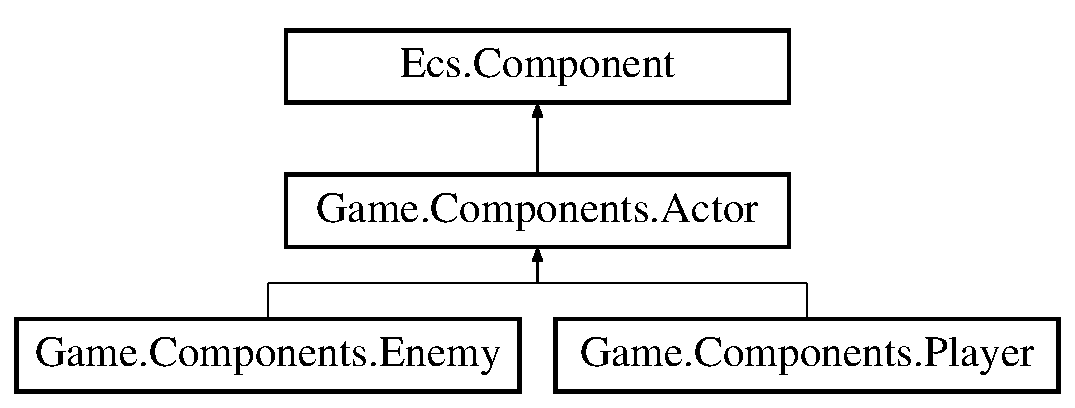
\includegraphics[height=3.000000cm]{class_game_1_1_components_1_1_actor}
\end{center}
\end{figure}
\subsection*{Public Member Functions}
\begin{DoxyCompactItemize}
\item 
\mbox{\Hypertarget{class_game_1_1_components_1_1_actor_a7ce72d5b0a98cf4c160e1f5fd24f880f}\label{class_game_1_1_components_1_1_actor_a7ce72d5b0a98cf4c160e1f5fd24f880f}} 
{\bfseries Actor} (string name, string description, int level, int hp, int arm, int attack)
\item 
\mbox{\Hypertarget{class_game_1_1_components_1_1_actor_ae23572d7be5ab106cfaed5907d8871e9}\label{class_game_1_1_components_1_1_actor_ae23572d7be5ab106cfaed5907d8871e9}} 
override void {\bfseries Start} ()
\item 
\mbox{\Hypertarget{class_game_1_1_components_1_1_actor_a947dffa306fa8a9cdcc33670de60dbb2}\label{class_game_1_1_components_1_1_actor_a947dffa306fa8a9cdcc33670de60dbb2}} 
override void {\bfseries Update} ()
\item 
\mbox{\Hypertarget{class_game_1_1_components_1_1_actor_a42d934f32a3090d2c4abb1f739c257c1}\label{class_game_1_1_components_1_1_actor_a42d934f32a3090d2c4abb1f739c257c1}} 
override void {\bfseries Render} ()
\end{DoxyCompactItemize}
\subsection*{Public Attributes}
\begin{DoxyCompactItemize}
\item 
\mbox{\Hypertarget{class_game_1_1_components_1_1_actor_ab33fef069cd89d2b95b1948fe7a0f1eb}\label{class_game_1_1_components_1_1_actor_ab33fef069cd89d2b95b1948fe7a0f1eb}} 
String {\bfseries name} = \char`\"{}\char`\"{}
\item 
\mbox{\Hypertarget{class_game_1_1_components_1_1_actor_a56d6ed805e0b74f0cf1c542f13b011a7}\label{class_game_1_1_components_1_1_actor_a56d6ed805e0b74f0cf1c542f13b011a7}} 
String {\bfseries description} = \char`\"{}\char`\"{}
\end{DoxyCompactItemize}
\subsection*{Protected Attributes}
\begin{DoxyCompactItemize}
\item 
\mbox{\Hypertarget{class_game_1_1_components_1_1_actor_a247427a6853d4195765fff7f44a0a6c4}\label{class_game_1_1_components_1_1_actor_a247427a6853d4195765fff7f44a0a6c4}} 
int {\bfseries hp} = 0
\item 
\mbox{\Hypertarget{class_game_1_1_components_1_1_actor_a4f53debbc0203e35cef271e4b94439f3}\label{class_game_1_1_components_1_1_actor_a4f53debbc0203e35cef271e4b94439f3}} 
int {\bfseries armor} = 0
\item 
\mbox{\Hypertarget{class_game_1_1_components_1_1_actor_a1fd6e57eab26c86802d6db3f88bd70c2}\label{class_game_1_1_components_1_1_actor_a1fd6e57eab26c86802d6db3f88bd70c2}} 
int {\bfseries attack} = 0
\item 
\mbox{\Hypertarget{class_game_1_1_components_1_1_actor_a84ca07cf456a329c6a3e1e6d4d9b3799}\label{class_game_1_1_components_1_1_actor_a84ca07cf456a329c6a3e1e6d4d9b3799}} 
int {\bfseries level} = 0
\end{DoxyCompactItemize}
\subsection*{Properties}
\begin{DoxyCompactItemize}
\item 
\mbox{\Hypertarget{class_game_1_1_components_1_1_actor_a61eb4ec857ac6ed3dacdc122cfbe438a}\label{class_game_1_1_components_1_1_actor_a61eb4ec857ac6ed3dacdc122cfbe438a}} 
int {\bfseries Hit\+Points}\hspace{0.3cm}{\ttfamily  \mbox{[}get\mbox{]}}
\item 
\mbox{\Hypertarget{class_game_1_1_components_1_1_actor_a502fd4fc55d418a847ef466bf09c96fa}\label{class_game_1_1_components_1_1_actor_a502fd4fc55d418a847ef466bf09c96fa}} 
int {\bfseries Armor}\hspace{0.3cm}{\ttfamily  \mbox{[}get\mbox{]}}
\item 
\mbox{\Hypertarget{class_game_1_1_components_1_1_actor_a244881aa54d3b73f74f09fb36e779837}\label{class_game_1_1_components_1_1_actor_a244881aa54d3b73f74f09fb36e779837}} 
String {\bfseries Name}\hspace{0.3cm}{\ttfamily  \mbox{[}get\mbox{]}}
\item 
\mbox{\Hypertarget{class_game_1_1_components_1_1_actor_aba6d2c82ffd258df393f4e08dbd74652}\label{class_game_1_1_components_1_1_actor_aba6d2c82ffd258df393f4e08dbd74652}} 
int {\bfseries Attack}\hspace{0.3cm}{\ttfamily  \mbox{[}get\mbox{]}}
\item 
\mbox{\Hypertarget{class_game_1_1_components_1_1_actor_aa3ea2c47b83cb50a7aaebe145a6b2f59}\label{class_game_1_1_components_1_1_actor_aa3ea2c47b83cb50a7aaebe145a6b2f59}} 
int {\bfseries Level}\hspace{0.3cm}{\ttfamily  \mbox{[}get\mbox{]}}
\end{DoxyCompactItemize}


The documentation for this class was generated from the following file\+:\begin{DoxyCompactItemize}
\item 
src/\+Game/\+Components/Actor.\+cs\end{DoxyCompactItemize}

\hypertarget{class_game_1_1_application}{}\section{Game.\+Application Class Reference}
\label{class_game_1_1_application}\index{Game.\+Application@{Game.\+Application}}
\subsection*{Public Member Functions}
\begin{DoxyCompactItemize}
\item 
\mbox{\Hypertarget{class_game_1_1_application_ac71b7eac1ed2ebc0d697d184428ca8e2}\label{class_game_1_1_application_ac71b7eac1ed2ebc0d697d184428ca8e2}} 
void {\bfseries Initialize} ()
\item 
\mbox{\Hypertarget{class_game_1_1_application_a53632a28eda450a69ad128d4914b56bf}\label{class_game_1_1_application_a53632a28eda450a69ad128d4914b56bf}} 
int {\bfseries Loop} ()
\item 
\mbox{\Hypertarget{class_game_1_1_application_a2ea7c18c0ee837403f7e8d4afeef30bc}\label{class_game_1_1_application_a2ea7c18c0ee837403f7e8d4afeef30bc}} 
void {\bfseries Update} ()
\item 
\mbox{\Hypertarget{class_game_1_1_application_a147214be44408796042eb1245bbd7f63}\label{class_game_1_1_application_a147214be44408796042eb1245bbd7f63}} 
void {\bfseries Render} ()
\end{DoxyCompactItemize}


The documentation for this class was generated from the following file\+:\begin{DoxyCompactItemize}
\item 
src/\+Game/Application.\+cs\end{DoxyCompactItemize}

\hypertarget{class_game_1_1_dungeon_maker_1_1_basic_dungeon}{}\section{Game.\+Dungeon\+Maker.\+Basic\+Dungeon Class Reference}
\label{class_game_1_1_dungeon_maker_1_1_basic_dungeon}\index{Game.\+Dungeon\+Maker.\+Basic\+Dungeon@{Game.\+Dungeon\+Maker.\+Basic\+Dungeon}}
\subsection*{Public Member Functions}
\begin{DoxyCompactItemize}
\item 
\mbox{\hyperlink{class_game_1_1_dungeon_maker_1_1_basic_dungeon_ae506d27631fab15f71cac7b3f20936c7}{Basic\+Dungeon}} (int width, int height, int seed)
\begin{DoxyCompactList}\small\item\em Creates a new empty dungeon of width and height dimensions using the seed provided. \end{DoxyCompactList}\item 
void \mbox{\hyperlink{class_game_1_1_dungeon_maker_1_1_basic_dungeon_ad9b7fb9bf2e0cdf3abfe49140168685e}{Generate}} ()
\begin{DoxyCompactList}\small\item\em Generates a dungeon based some ideas described by Bob Nystrom in his wonderful article \char`\"{}\+Rooms and Mazes\char`\"{}. \href{http://journal.stuffwithstuff.com/2014/12/21/rooms-and-mazes/with}{\tt http\+://journal.\+stuffwithstuff.\+com/2014/12/21/rooms-\/and-\/mazes/with} \end{DoxyCompactList}\item 
void \mbox{\hyperlink{class_game_1_1_dungeon_maker_1_1_basic_dungeon_a2cf2d36643ff09242016a187bf29dcdf}{Draw}} ()
\begin{DoxyCompactList}\small\item\em Debug function to draw the dungeon to the screen. Note that the output may not fit on the screen. \end{DoxyCompactList}\item 
List$<$ String $>$ \mbox{\hyperlink{class_game_1_1_dungeon_maker_1_1_basic_dungeon_a5ea4d65fbdf434976300b6e655d8b8d0}{Stringify}} ()
\begin{DoxyCompactList}\small\item\em Converts the dungeon into a list of string rows for use in the {\ttfamily Model} class. \end{DoxyCompactList}\item 
\mbox{\Hypertarget{class_game_1_1_dungeon_maker_1_1_basic_dungeon_a4c460b2fbd9124ebad23ea425e0f94d0}\label{class_game_1_1_dungeon_maker_1_1_basic_dungeon_a4c460b2fbd9124ebad23ea425e0f94d0}} 
List$<$ List$<$ String $>$ $>$ {\bfseries Package} ()
\end{DoxyCompactItemize}


\subsection{Constructor \& Destructor Documentation}
\mbox{\Hypertarget{class_game_1_1_dungeon_maker_1_1_basic_dungeon_ae506d27631fab15f71cac7b3f20936c7}\label{class_game_1_1_dungeon_maker_1_1_basic_dungeon_ae506d27631fab15f71cac7b3f20936c7}} 
\index{Game\+::\+Dungeon\+Maker\+::\+Basic\+Dungeon@{Game\+::\+Dungeon\+Maker\+::\+Basic\+Dungeon}!Basic\+Dungeon@{Basic\+Dungeon}}
\index{Basic\+Dungeon@{Basic\+Dungeon}!Game\+::\+Dungeon\+Maker\+::\+Basic\+Dungeon@{Game\+::\+Dungeon\+Maker\+::\+Basic\+Dungeon}}
\subsubsection{\texorpdfstring{Basic\+Dungeon()}{BasicDungeon()}}
{\footnotesize\ttfamily Game.\+Dungeon\+Maker.\+Basic\+Dungeon.\+Basic\+Dungeon (\begin{DoxyParamCaption}\item[{int}]{width,  }\item[{int}]{height,  }\item[{int}]{seed }\end{DoxyParamCaption})}



Creates a new empty dungeon of width and height dimensions using the seed provided. 


\begin{DoxyParams}{Parameters}
{\em width} & Width of the dungeon\\
\hline
{\em height} & Height of the dungeon\\
\hline
{\em seed} & Unique seed used to generate and place rooms. Generation is also dependent on height/width combination.\\
\hline
\end{DoxyParams}


\subsection{Member Function Documentation}
\mbox{\Hypertarget{class_game_1_1_dungeon_maker_1_1_basic_dungeon_a2cf2d36643ff09242016a187bf29dcdf}\label{class_game_1_1_dungeon_maker_1_1_basic_dungeon_a2cf2d36643ff09242016a187bf29dcdf}} 
\index{Game\+::\+Dungeon\+Maker\+::\+Basic\+Dungeon@{Game\+::\+Dungeon\+Maker\+::\+Basic\+Dungeon}!Draw@{Draw}}
\index{Draw@{Draw}!Game\+::\+Dungeon\+Maker\+::\+Basic\+Dungeon@{Game\+::\+Dungeon\+Maker\+::\+Basic\+Dungeon}}
\subsubsection{\texorpdfstring{Draw()}{Draw()}}
{\footnotesize\ttfamily void Game.\+Dungeon\+Maker.\+Basic\+Dungeon.\+Draw (\begin{DoxyParamCaption}{ }\end{DoxyParamCaption})}



Debug function to draw the dungeon to the screen. Note that the output may not fit on the screen. 

\mbox{\Hypertarget{class_game_1_1_dungeon_maker_1_1_basic_dungeon_ad9b7fb9bf2e0cdf3abfe49140168685e}\label{class_game_1_1_dungeon_maker_1_1_basic_dungeon_ad9b7fb9bf2e0cdf3abfe49140168685e}} 
\index{Game\+::\+Dungeon\+Maker\+::\+Basic\+Dungeon@{Game\+::\+Dungeon\+Maker\+::\+Basic\+Dungeon}!Generate@{Generate}}
\index{Generate@{Generate}!Game\+::\+Dungeon\+Maker\+::\+Basic\+Dungeon@{Game\+::\+Dungeon\+Maker\+::\+Basic\+Dungeon}}
\subsubsection{\texorpdfstring{Generate()}{Generate()}}
{\footnotesize\ttfamily void Game.\+Dungeon\+Maker.\+Basic\+Dungeon.\+Generate (\begin{DoxyParamCaption}{ }\end{DoxyParamCaption})}



Generates a dungeon based some ideas described by Bob Nystrom in his wonderful article \char`\"{}\+Rooms and Mazes\char`\"{}. \href{http://journal.stuffwithstuff.com/2014/12/21/rooms-and-mazes/with}{\tt http\+://journal.\+stuffwithstuff.\+com/2014/12/21/rooms-\/and-\/mazes/with} 

\mbox{\Hypertarget{class_game_1_1_dungeon_maker_1_1_basic_dungeon_a5ea4d65fbdf434976300b6e655d8b8d0}\label{class_game_1_1_dungeon_maker_1_1_basic_dungeon_a5ea4d65fbdf434976300b6e655d8b8d0}} 
\index{Game\+::\+Dungeon\+Maker\+::\+Basic\+Dungeon@{Game\+::\+Dungeon\+Maker\+::\+Basic\+Dungeon}!Stringify@{Stringify}}
\index{Stringify@{Stringify}!Game\+::\+Dungeon\+Maker\+::\+Basic\+Dungeon@{Game\+::\+Dungeon\+Maker\+::\+Basic\+Dungeon}}
\subsubsection{\texorpdfstring{Stringify()}{Stringify()}}
{\footnotesize\ttfamily List$<$String$>$ Game.\+Dungeon\+Maker.\+Basic\+Dungeon.\+Stringify (\begin{DoxyParamCaption}{ }\end{DoxyParamCaption})}



Converts the dungeon into a list of string rows for use in the {\ttfamily Model} class. 

\begin{DoxyReturn}{Returns}

\end{DoxyReturn}


The documentation for this class was generated from the following file\+:\begin{DoxyCompactItemize}
\item 
src/\+Game/\+Dungeon\+Maker/Basic\+Dungeon.\+cs\end{DoxyCompactItemize}

\hypertarget{class_game_1_1_dungeon_maker_1_1_cell}{}\section{Game.\+Dungeon\+Maker.\+Cell Class Reference}
\label{class_game_1_1_dungeon_maker_1_1_cell}\index{Game.\+Dungeon\+Maker.\+Cell@{Game.\+Dungeon\+Maker.\+Cell}}
\subsection*{Public Member Functions}
\begin{DoxyCompactItemize}
\item 
\mbox{\hyperlink{class_game_1_1_dungeon_maker_1_1_cell_a172d3f97d797bba46dd27cf2e5c04c87}{Cell}} ()
\begin{DoxyCompactList}\small\item\em A representation of one square on the map, which can be one of several types. \end{DoxyCompactList}\item 
bool \mbox{\hyperlink{class_game_1_1_dungeon_maker_1_1_cell_aef83c7358aea7dfc626b2375de6848d1}{Is\+Open}} ()
\begin{DoxyCompactList}\small\item\em Checks whether a cell is solid wall or not. \end{DoxyCompactList}\item 
String \mbox{\hyperlink{class_game_1_1_dungeon_maker_1_1_cell_ad3b5ac0a0e3376f1661b35c4d10c5116}{To\+Char}} ()
\begin{DoxyCompactList}\small\item\em Gets a string representation of the cell, depending on its type. \end{DoxyCompactList}\end{DoxyCompactItemize}
\subsection*{Public Attributes}
\begin{DoxyCompactItemize}
\item 
\mbox{\Hypertarget{class_game_1_1_dungeon_maker_1_1_cell_a85570a8a7505dcf10261d0f98a47245c}\label{class_game_1_1_dungeon_maker_1_1_cell_a85570a8a7505dcf10261d0f98a47245c}} 
Cell\+Type {\bfseries type} = Cell\+Type.\+Wall
\item 
\mbox{\Hypertarget{class_game_1_1_dungeon_maker_1_1_cell_a5790b92b6a3eefebf7e2e3a0667233b8}\label{class_game_1_1_dungeon_maker_1_1_cell_a5790b92b6a3eefebf7e2e3a0667233b8}} 
int {\bfseries group} = 0
\end{DoxyCompactItemize}


\subsection{Constructor \& Destructor Documentation}
\mbox{\Hypertarget{class_game_1_1_dungeon_maker_1_1_cell_a172d3f97d797bba46dd27cf2e5c04c87}\label{class_game_1_1_dungeon_maker_1_1_cell_a172d3f97d797bba46dd27cf2e5c04c87}} 
\index{Game\+::\+Dungeon\+Maker\+::\+Cell@{Game\+::\+Dungeon\+Maker\+::\+Cell}!Cell@{Cell}}
\index{Cell@{Cell}!Game\+::\+Dungeon\+Maker\+::\+Cell@{Game\+::\+Dungeon\+Maker\+::\+Cell}}
\subsubsection{\texorpdfstring{Cell()}{Cell()}}
{\footnotesize\ttfamily Game.\+Dungeon\+Maker.\+Cell.\+Cell (\begin{DoxyParamCaption}{ }\end{DoxyParamCaption})}



A representation of one square on the map, which can be one of several types. 



\subsection{Member Function Documentation}
\mbox{\Hypertarget{class_game_1_1_dungeon_maker_1_1_cell_aef83c7358aea7dfc626b2375de6848d1}\label{class_game_1_1_dungeon_maker_1_1_cell_aef83c7358aea7dfc626b2375de6848d1}} 
\index{Game\+::\+Dungeon\+Maker\+::\+Cell@{Game\+::\+Dungeon\+Maker\+::\+Cell}!Is\+Open@{Is\+Open}}
\index{Is\+Open@{Is\+Open}!Game\+::\+Dungeon\+Maker\+::\+Cell@{Game\+::\+Dungeon\+Maker\+::\+Cell}}
\subsubsection{\texorpdfstring{Is\+Open()}{IsOpen()}}
{\footnotesize\ttfamily bool Game.\+Dungeon\+Maker.\+Cell.\+Is\+Open (\begin{DoxyParamCaption}{ }\end{DoxyParamCaption})}



Checks whether a cell is solid wall or not. 

\begin{DoxyReturn}{Returns}
Returns true if the cell is a room passage or door.
\end{DoxyReturn}
\mbox{\Hypertarget{class_game_1_1_dungeon_maker_1_1_cell_ad3b5ac0a0e3376f1661b35c4d10c5116}\label{class_game_1_1_dungeon_maker_1_1_cell_ad3b5ac0a0e3376f1661b35c4d10c5116}} 
\index{Game\+::\+Dungeon\+Maker\+::\+Cell@{Game\+::\+Dungeon\+Maker\+::\+Cell}!To\+Char@{To\+Char}}
\index{To\+Char@{To\+Char}!Game\+::\+Dungeon\+Maker\+::\+Cell@{Game\+::\+Dungeon\+Maker\+::\+Cell}}
\subsubsection{\texorpdfstring{To\+Char()}{ToChar()}}
{\footnotesize\ttfamily String Game.\+Dungeon\+Maker.\+Cell.\+To\+Char (\begin{DoxyParamCaption}{ }\end{DoxyParamCaption})}



Gets a string representation of the cell, depending on its type. 

\begin{DoxyReturn}{Returns}
Returns a one-\/character representation.
\end{DoxyReturn}


The documentation for this class was generated from the following file\+:\begin{DoxyCompactItemize}
\item 
src/\+Game/\+Dungeon\+Maker/Cell.\+cs\end{DoxyCompactItemize}

\hypertarget{class_game_1_1_components_1_1_collider}{}\section{Game.\+Components.\+Collider Class Reference}
\label{class_game_1_1_components_1_1_collider}\index{Game.\+Components.\+Collider@{Game.\+Components.\+Collider}}
Inheritance diagram for Game.\+Components.\+Collider\+:\begin{figure}[H]
\begin{center}
\leavevmode
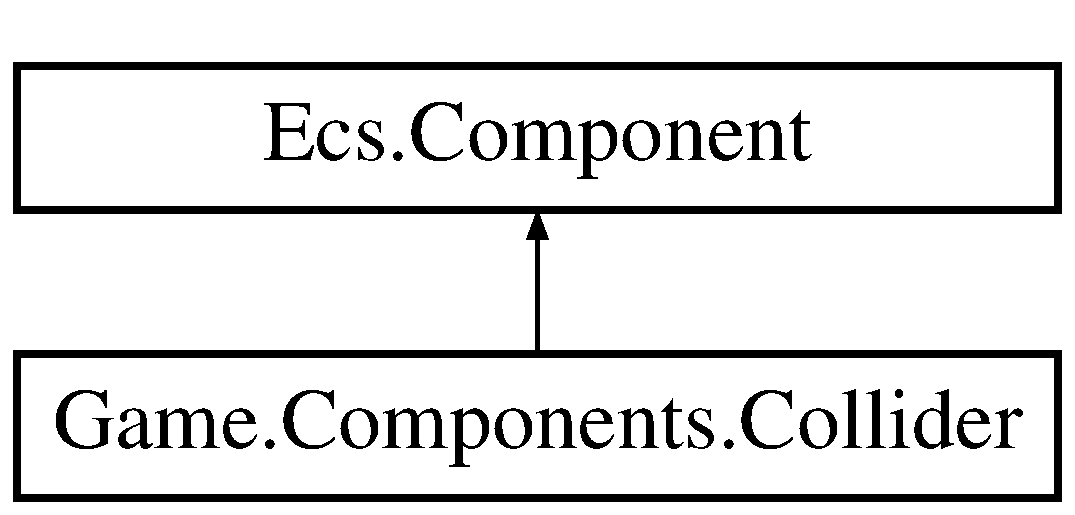
\includegraphics[height=2.000000cm]{class_game_1_1_components_1_1_collider}
\end{center}
\end{figure}
\subsection*{Public Member Functions}
\begin{DoxyCompactItemize}
\item 
\mbox{\Hypertarget{class_game_1_1_components_1_1_collider_a95f93ad13110b536fa365faed0fe4593}\label{class_game_1_1_components_1_1_collider_a95f93ad13110b536fa365faed0fe4593}} 
override void {\bfseries Start} ()
\item 
\mbox{\Hypertarget{class_game_1_1_components_1_1_collider_aa60b9a14541bc5beff644c9fe44ce313}\label{class_game_1_1_components_1_1_collider_aa60b9a14541bc5beff644c9fe44ce313}} 
override void {\bfseries Update} ()
\item 
\mbox{\Hypertarget{class_game_1_1_components_1_1_collider_a58566e658035ac726fa8d5587ece5ded}\label{class_game_1_1_components_1_1_collider_a58566e658035ac726fa8d5587ece5ded}} 
override void {\bfseries Render} ()
\item 
\mbox{\hyperlink{namespace_game_1_1_data_structures_ada1f9e4784b55145987867a5daf71d4d}{Collision\+Types}} \mbox{\hyperlink{class_game_1_1_components_1_1_collider_a4b9f921f8563cdccd1b0dbf9664cc08f}{Handle\+Collision}} (int dx, int dy, out \mbox{\hyperlink{class_ecs_1_1_game_object}{Game\+Object}} found)
\begin{DoxyCompactList}\small\item\em Uses an inputted movement and uses the current position and the movement to check if there location being moved into is empty or not. If there is already a game object at that spot, it will also return a reference to that game object. \end{DoxyCompactList}\end{DoxyCompactItemize}
\subsection*{Additional Inherited Members}


\subsection{Member Function Documentation}
\mbox{\Hypertarget{class_game_1_1_components_1_1_collider_a4b9f921f8563cdccd1b0dbf9664cc08f}\label{class_game_1_1_components_1_1_collider_a4b9f921f8563cdccd1b0dbf9664cc08f}} 
\index{Game\+::\+Components\+::\+Collider@{Game\+::\+Components\+::\+Collider}!Handle\+Collision@{Handle\+Collision}}
\index{Handle\+Collision@{Handle\+Collision}!Game\+::\+Components\+::\+Collider@{Game\+::\+Components\+::\+Collider}}
\subsubsection{\texorpdfstring{Handle\+Collision()}{HandleCollision()}}
{\footnotesize\ttfamily \mbox{\hyperlink{namespace_game_1_1_data_structures_ada1f9e4784b55145987867a5daf71d4d}{Collision\+Types}} Game.\+Components.\+Collider.\+Handle\+Collision (\begin{DoxyParamCaption}\item[{int}]{dx,  }\item[{int}]{dy,  }\item[{out \mbox{\hyperlink{class_ecs_1_1_game_object}{Game\+Object}}}]{found }\end{DoxyParamCaption})}



Uses an inputted movement and uses the current position and the movement to check if there location being moved into is empty or not. If there is already a game object at that spot, it will also return a reference to that game object. 


\begin{DoxyParams}{Parameters}
{\em dx} & \\
\hline
{\em dy} & \\
\hline
{\em found} & \\
\hline
\end{DoxyParams}
\begin{DoxyReturn}{Returns}

\end{DoxyReturn}


The documentation for this class was generated from the following file\+:\begin{DoxyCompactItemize}
\item 
src/\+Game/\+Components/Collider.\+cs\end{DoxyCompactItemize}

\hypertarget{class_ecs_1_1_component}{}\section{Ecs.\+Component Class Reference}
\label{class_ecs_1_1_component}\index{Ecs.\+Component@{Ecs.\+Component}}
Inheritance diagram for Ecs.\+Component\+:\begin{figure}[H]
\begin{center}
\leavevmode
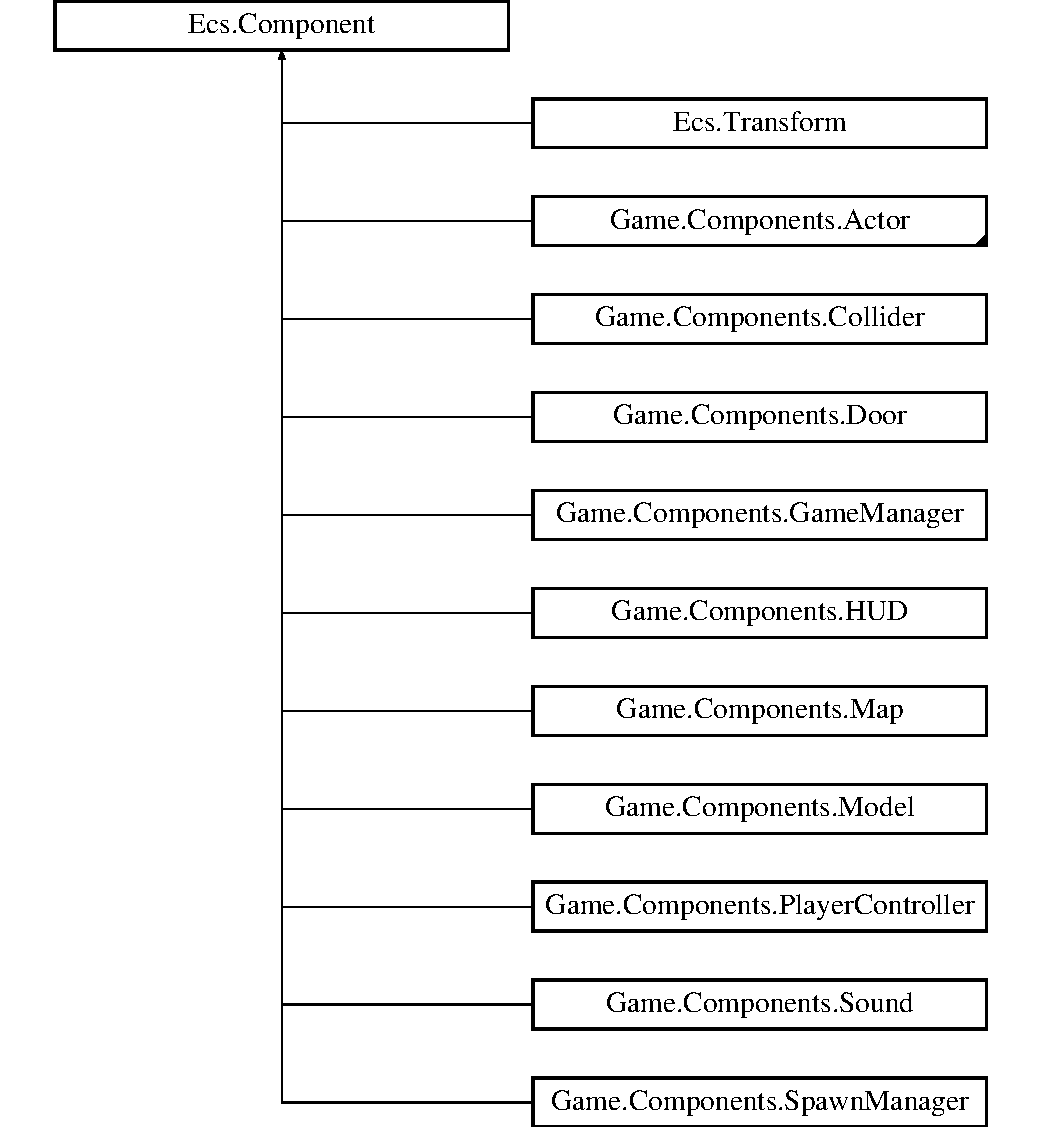
\includegraphics[height=12.000000cm]{class_ecs_1_1_component}
\end{center}
\end{figure}
\subsection*{Public Member Functions}
\begin{DoxyCompactItemize}
\item 
\mbox{\Hypertarget{class_ecs_1_1_component_ad19efc33f8968ba433aef4df8d4e5488}\label{class_ecs_1_1_component_ad19efc33f8968ba433aef4df8d4e5488}} 
virtual void {\bfseries Start} ()
\item 
\mbox{\Hypertarget{class_ecs_1_1_component_ac921cd8d6108a93deabb1b01d21899df}\label{class_ecs_1_1_component_ac921cd8d6108a93deabb1b01d21899df}} 
virtual void {\bfseries Update} ()
\item 
\mbox{\Hypertarget{class_ecs_1_1_component_a44e8b62ae33a573ba0a00b44528599ad}\label{class_ecs_1_1_component_a44e8b62ae33a573ba0a00b44528599ad}} 
virtual void {\bfseries Late\+Update} ()
\item 
\mbox{\Hypertarget{class_ecs_1_1_component_ab11b3633f26ba2a465a02cec6d71cb9e}\label{class_ecs_1_1_component_ab11b3633f26ba2a465a02cec6d71cb9e}} 
virtual void {\bfseries Render} ()
\item 
\mbox{\Hypertarget{class_ecs_1_1_component_a6408efbaf664274ce4d33e7484627180}\label{class_ecs_1_1_component_a6408efbaf664274ce4d33e7484627180}} 
virtual void {\bfseries On\+Enable} ()
\item 
\mbox{\Hypertarget{class_ecs_1_1_component_a1583b54e365b28288ecc86684650ec2d}\label{class_ecs_1_1_component_a1583b54e365b28288ecc86684650ec2d}} 
virtual void {\bfseries On\+Disable} ()
\item 
\mbox{\Hypertarget{class_ecs_1_1_component_a5a8a74654c295f63cb943948638cd392}\label{class_ecs_1_1_component_a5a8a74654c295f63cb943948638cd392}} 
\mbox{\hyperlink{class_ecs_1_1_component}{Component}} {\bfseries Get\+Component} (Type type)
\item 
\mbox{\Hypertarget{class_ecs_1_1_component_a5f86d9053da960b2e8c2784af7b1660e}\label{class_ecs_1_1_component_a5f86d9053da960b2e8c2784af7b1660e}} 
\mbox{\hyperlink{class_ecs_1_1_component}{Component}} {\bfseries Get\+Component$<$ T $>$} ()
\item 
\mbox{\Hypertarget{class_ecs_1_1_component_a8854b7791f9dc6d8d9ec95e79c10355a}\label{class_ecs_1_1_component_a8854b7791f9dc6d8d9ec95e79c10355a}} 
\mbox{\hyperlink{class_ecs_1_1_component}{Component}} {\bfseries Get\+Component\+In\+Children$<$ T $>$} ()
\item 
\mbox{\Hypertarget{class_ecs_1_1_component_a20ea1d6cf3fb9ed8726b041d1ca20a29}\label{class_ecs_1_1_component_a20ea1d6cf3fb9ed8726b041d1ca20a29}} 
\mbox{\hyperlink{class_ecs_1_1_component}{Component}} {\bfseries Add\+Component} (\mbox{\hyperlink{class_ecs_1_1_component}{Component}} component)
\item 
\mbox{\Hypertarget{class_ecs_1_1_component_a6a34a62ab59f8f15ae015d7526682c32}\label{class_ecs_1_1_component_a6a34a62ab59f8f15ae015d7526682c32}} 
\mbox{\hyperlink{class_ecs_1_1_component}{Component}} {\bfseries Add\+Component$<$ T $>$} ()
\item 
\mbox{\Hypertarget{class_ecs_1_1_component_ab9256d060b3c50c44b53d1b37c27eeac}\label{class_ecs_1_1_component_ab9256d060b3c50c44b53d1b37c27eeac}} 
bool {\bfseries Is\+Active} ()
\item 
\mbox{\Hypertarget{class_ecs_1_1_component_a8b3f556d3c3318f2df4bb0062a5a40e3}\label{class_ecs_1_1_component_a8b3f556d3c3318f2df4bb0062a5a40e3}} 
void {\bfseries Set\+Active} (bool active)
\end{DoxyCompactItemize}
\subsection*{Public Attributes}
\begin{DoxyCompactItemize}
\item 
\mbox{\Hypertarget{class_ecs_1_1_component_a07e9056497ace18a151c4ae9e2938798}\label{class_ecs_1_1_component_a07e9056497ace18a151c4ae9e2938798}} 
\mbox{\hyperlink{class_ecs_1_1_game_object}{Game\+Object}} {\bfseries game\+Object} = null
\item 
\mbox{\Hypertarget{class_ecs_1_1_component_a13b68c9cce3ae3fd514dcedc1edd595a}\label{class_ecs_1_1_component_a13b68c9cce3ae3fd514dcedc1edd595a}} 
\mbox{\hyperlink{class_ecs_1_1_transform}{Transform}} {\bfseries transform} = null
\end{DoxyCompactItemize}


The documentation for this class was generated from the following file\+:\begin{DoxyCompactItemize}
\item 
src/\+Ecs/Component.\+cs\end{DoxyCompactItemize}

\hypertarget{class_i_o_1_1_console_u_i}{}\section{I\+O.\+Console\+UI Class Reference}
\label{class_i_o_1_1_console_u_i}\index{I\+O.\+Console\+UI@{I\+O.\+Console\+UI}}
\subsection*{Public Member Functions}
\begin{DoxyCompactItemize}
\item 
\mbox{\Hypertarget{class_i_o_1_1_console_u_i_a0c7f62392769a5d8f3eb557a69dfaa4e}\label{class_i_o_1_1_console_u_i_a0c7f62392769a5d8f3eb557a69dfaa4e}} 
static uint {\bfseries Get\+Last\+Error} ()
\end{DoxyCompactItemize}
\subsection*{Static Public Member Functions}
\begin{DoxyCompactItemize}
\item 
\mbox{\Hypertarget{class_i_o_1_1_console_u_i_a3969348ad591fb8bd0b0a5ac9cb08a9e}\label{class_i_o_1_1_console_u_i_a3969348ad591fb8bd0b0a5ac9cb08a9e}} 
static void {\bfseries Initialize} (int new\+Width, int new\+Height)
\item 
static void \mbox{\hyperlink{class_i_o_1_1_console_u_i_a7b605726f9cc6c04e7656ffe1efa50f0}{Clear\+Buffer}} ()
\begin{DoxyCompactList}\small\item\em Clear the contents of the buffer string table. Reset the screen contents with default draw box. \end{DoxyCompactList}\item 
static void \mbox{\hyperlink{class_i_o_1_1_console_u_i_a8fe3234db68da3a6b652446f317f92cd}{Render}} ()
\begin{DoxyCompactList}\small\item\em Draw everything from the buffer to the console. \end{DoxyCompactList}\item 
\mbox{\Hypertarget{class_i_o_1_1_console_u_i_ae6befc1153f02e49bc37b80279b5ca24}\label{class_i_o_1_1_console_u_i_ae6befc1153f02e49bc37b80279b5ca24}} 
static void {\bfseries Write} (int x, int y, char output, String color=default\+Color)
\item 
\mbox{\Hypertarget{class_i_o_1_1_console_u_i_a9a5389eab5915fefa39f0113bbdb22ee}\label{class_i_o_1_1_console_u_i_a9a5389eab5915fefa39f0113bbdb22ee}} 
static void {\bfseries Write} (int x, int y, String output, List$<$ String $>$ colors=null)
\item 
\mbox{\Hypertarget{class_i_o_1_1_console_u_i_a5a140bb45584b0876d4cd05af1f029f2}\label{class_i_o_1_1_console_u_i_a5a140bb45584b0876d4cd05af1f029f2}} 
static void {\bfseries Write} (int x, int y, List$<$ String $>$ lines, List$<$ List$<$ String $>$$>$ colors=null)
\item 
\mbox{\Hypertarget{class_i_o_1_1_console_u_i_acc2e309427aa386d947d0f22f3ee3b4a}\label{class_i_o_1_1_console_u_i_acc2e309427aa386d947d0f22f3ee3b4a}} 
static int {\bfseries Max\+Width} ()
\item 
\mbox{\Hypertarget{class_i_o_1_1_console_u_i_a23b24ed44e1b7d603706af686f04c81e}\label{class_i_o_1_1_console_u_i_a23b24ed44e1b7d603706af686f04c81e}} 
static int {\bfseries Max\+Height} ()
\end{DoxyCompactItemize}


\subsection{Member Function Documentation}
\mbox{\Hypertarget{class_i_o_1_1_console_u_i_a7b605726f9cc6c04e7656ffe1efa50f0}\label{class_i_o_1_1_console_u_i_a7b605726f9cc6c04e7656ffe1efa50f0}} 
\index{I\+O\+::\+Console\+UI@{I\+O\+::\+Console\+UI}!Clear\+Buffer@{Clear\+Buffer}}
\index{Clear\+Buffer@{Clear\+Buffer}!I\+O\+::\+Console\+UI@{I\+O\+::\+Console\+UI}}
\subsubsection{\texorpdfstring{Clear\+Buffer()}{ClearBuffer()}}
{\footnotesize\ttfamily static void I\+O.\+Console\+U\+I.\+Clear\+Buffer (\begin{DoxyParamCaption}{ }\end{DoxyParamCaption})\hspace{0.3cm}{\ttfamily [static]}}



Clear the contents of the buffer string table. Reset the screen contents with default draw box. 

\mbox{\Hypertarget{class_i_o_1_1_console_u_i_a8fe3234db68da3a6b652446f317f92cd}\label{class_i_o_1_1_console_u_i_a8fe3234db68da3a6b652446f317f92cd}} 
\index{I\+O\+::\+Console\+UI@{I\+O\+::\+Console\+UI}!Render@{Render}}
\index{Render@{Render}!I\+O\+::\+Console\+UI@{I\+O\+::\+Console\+UI}}
\subsubsection{\texorpdfstring{Render()}{Render()}}
{\footnotesize\ttfamily static void I\+O.\+Console\+U\+I.\+Render (\begin{DoxyParamCaption}{ }\end{DoxyParamCaption})\hspace{0.3cm}{\ttfamily [static]}}



Draw everything from the buffer to the console. 



The documentation for this class was generated from the following file\+:\begin{DoxyCompactItemize}
\item 
src/\+I\+O/Console\+U\+I.\+cs\end{DoxyCompactItemize}

\hypertarget{class_game_1_1_dungeon_maker_1_1_coord}{}\section{Game.\+Dungeon\+Maker.\+Coord Class Reference}
\label{class_game_1_1_dungeon_maker_1_1_coord}\index{Game.\+Dungeon\+Maker.\+Coord@{Game.\+Dungeon\+Maker.\+Coord}}
\subsection*{Public Member Functions}
\begin{DoxyCompactItemize}
\item 
\mbox{\hyperlink{class_game_1_1_dungeon_maker_1_1_coord_ab8f7b0486b1be73445e2f004d8d75426}{Coord}} (int x, int y)
\begin{DoxyCompactList}\small\item\em Creates a x/y coordinate pair. Mainly for use in Lists. \end{DoxyCompactList}\end{DoxyCompactItemize}
\subsection*{Public Attributes}
\begin{DoxyCompactItemize}
\item 
\mbox{\Hypertarget{class_game_1_1_dungeon_maker_1_1_coord_ae52fb2527e23cd0c695632fdcb9926ff}\label{class_game_1_1_dungeon_maker_1_1_coord_ae52fb2527e23cd0c695632fdcb9926ff}} 
int {\bfseries x}
\item 
\mbox{\Hypertarget{class_game_1_1_dungeon_maker_1_1_coord_aa24f6d2ab099e02d19560bc69b5c0bdf}\label{class_game_1_1_dungeon_maker_1_1_coord_aa24f6d2ab099e02d19560bc69b5c0bdf}} 
int {\bfseries y}
\end{DoxyCompactItemize}


\subsection{Constructor \& Destructor Documentation}
\mbox{\Hypertarget{class_game_1_1_dungeon_maker_1_1_coord_ab8f7b0486b1be73445e2f004d8d75426}\label{class_game_1_1_dungeon_maker_1_1_coord_ab8f7b0486b1be73445e2f004d8d75426}} 
\index{Game\+::\+Dungeon\+Maker\+::\+Coord@{Game\+::\+Dungeon\+Maker\+::\+Coord}!Coord@{Coord}}
\index{Coord@{Coord}!Game\+::\+Dungeon\+Maker\+::\+Coord@{Game\+::\+Dungeon\+Maker\+::\+Coord}}
\subsubsection{\texorpdfstring{Coord()}{Coord()}}
{\footnotesize\ttfamily Game.\+Dungeon\+Maker.\+Coord.\+Coord (\begin{DoxyParamCaption}\item[{int}]{x,  }\item[{int}]{y }\end{DoxyParamCaption})}



Creates a x/y coordinate pair. Mainly for use in Lists. 


\begin{DoxyParams}{Parameters}
{\em x} & X coordinate\\
\hline
{\em y} & Y coordinate\\
\hline
\end{DoxyParams}


The documentation for this class was generated from the following file\+:\begin{DoxyCompactItemize}
\item 
src/\+Game/\+Dungeon\+Maker/Coord.\+cs\end{DoxyCompactItemize}

\hypertarget{class_i_o_1_1_debug}{}\section{I\+O.\+Debug Class Reference}
\label{class_i_o_1_1_debug}\index{I\+O.\+Debug@{I\+O.\+Debug}}
\subsection*{Static Public Member Functions}
\begin{DoxyCompactItemize}
\item 
\mbox{\Hypertarget{class_i_o_1_1_debug_af4e5c954d9c5df29b4936fdfb388bb57}\label{class_i_o_1_1_debug_af4e5c954d9c5df29b4936fdfb388bb57}} 
static void {\bfseries Log} (string log)
\item 
\mbox{\Hypertarget{class_i_o_1_1_debug_a64e7869062d1bb94006b1174673ac36b}\label{class_i_o_1_1_debug_a64e7869062d1bb94006b1174673ac36b}} 
static void {\bfseries Log\+Warning} (string warning)
\item 
\mbox{\Hypertarget{class_i_o_1_1_debug_a0c08a7c31a3d9b91cef8e87a832326a2}\label{class_i_o_1_1_debug_a0c08a7c31a3d9b91cef8e87a832326a2}} 
static void {\bfseries Log\+Error} (string error)
\end{DoxyCompactItemize}


The documentation for this class was generated from the following file\+:\begin{DoxyCompactItemize}
\item 
src/\+I\+O/Debug.\+cs\end{DoxyCompactItemize}

\hypertarget{class_game_1_1_components_1_1_door}{}\section{Game.\+Components.\+Door Class Reference}
\label{class_game_1_1_components_1_1_door}\index{Game.\+Components.\+Door@{Game.\+Components.\+Door}}
Inheritance diagram for Game.\+Components.\+Door\+:\begin{figure}[H]
\begin{center}
\leavevmode
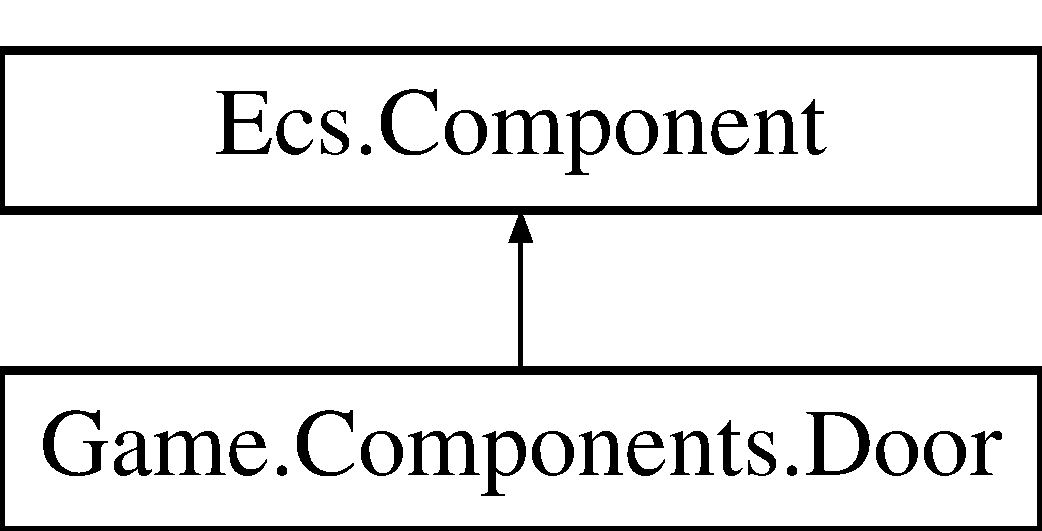
\includegraphics[height=2.000000cm]{class_game_1_1_components_1_1_door}
\end{center}
\end{figure}
\subsection*{Public Member Functions}
\begin{DoxyCompactItemize}
\item 
\mbox{\Hypertarget{class_game_1_1_components_1_1_door_ac04bdfb1dadbe9592cb13e0e88de63e1}\label{class_game_1_1_components_1_1_door_ac04bdfb1dadbe9592cb13e0e88de63e1}} 
override void {\bfseries Start} ()
\item 
\mbox{\Hypertarget{class_game_1_1_components_1_1_door_a0c075c913385dd33fe981f47caa94de7}\label{class_game_1_1_components_1_1_door_a0c075c913385dd33fe981f47caa94de7}} 
override void {\bfseries Update} ()
\item 
\mbox{\Hypertarget{class_game_1_1_components_1_1_door_a50acad4b65a94f7544b383d6c8b0fed7}\label{class_game_1_1_components_1_1_door_a50acad4b65a94f7544b383d6c8b0fed7}} 
override void {\bfseries Render} ()
\end{DoxyCompactItemize}
\subsection*{Additional Inherited Members}


The documentation for this class was generated from the following file\+:\begin{DoxyCompactItemize}
\item 
src/\+Game/\+Components/Door.\+cs\end{DoxyCompactItemize}

\hypertarget{class_game_1_1_components_1_1_enemy}{}\section{Game.\+Components.\+Enemy Class Reference}
\label{class_game_1_1_components_1_1_enemy}\index{Game.\+Components.\+Enemy@{Game.\+Components.\+Enemy}}
Inheritance diagram for Game.\+Components.\+Enemy\+:\begin{figure}[H]
\begin{center}
\leavevmode
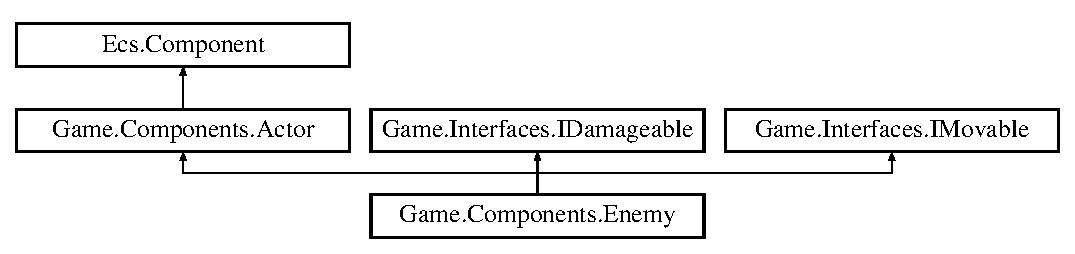
\includegraphics[height=2.962963cm]{class_game_1_1_components_1_1_enemy}
\end{center}
\end{figure}
\subsection*{Public Member Functions}
\begin{DoxyCompactItemize}
\item 
\mbox{\Hypertarget{class_game_1_1_components_1_1_enemy_a109666b6285493ec597aca97a3a842f9}\label{class_game_1_1_components_1_1_enemy_a109666b6285493ec597aca97a3a842f9}} 
{\bfseries Enemy} (string name, string description, int level, int hp, int arm, int attack, int rate)
\item 
\mbox{\Hypertarget{class_game_1_1_components_1_1_enemy_ab2cea47dab16b552b9be2c0c13d078fb}\label{class_game_1_1_components_1_1_enemy_ab2cea47dab16b552b9be2c0c13d078fb}} 
override void {\bfseries Start} ()
\item 
\mbox{\Hypertarget{class_game_1_1_components_1_1_enemy_a2f1d9495e7b2860044a34dff789f5b89}\label{class_game_1_1_components_1_1_enemy_a2f1d9495e7b2860044a34dff789f5b89}} 
override void {\bfseries Update} ()
\item 
\mbox{\Hypertarget{class_game_1_1_components_1_1_enemy_a0e561eb1bcce3e1a66fcd973d02982f6}\label{class_game_1_1_components_1_1_enemy_a0e561eb1bcce3e1a66fcd973d02982f6}} 
override void {\bfseries Render} ()
\item 
\mbox{\Hypertarget{class_game_1_1_components_1_1_enemy_af6d1357b07693138ca315f5064f22de1}\label{class_game_1_1_components_1_1_enemy_af6d1357b07693138ca315f5064f22de1}} 
void {\bfseries Apply\+Damage} (int damage)
\item 
\mbox{\Hypertarget{class_game_1_1_components_1_1_enemy_a084693a2505f011fa8c8103ecd01a126}\label{class_game_1_1_components_1_1_enemy_a084693a2505f011fa8c8103ecd01a126}} 
void {\bfseries On\+Death} ()
\item 
\mbox{\Hypertarget{class_game_1_1_components_1_1_enemy_a2021a5a82cf1ce9c90b3433f5d304283}\label{class_game_1_1_components_1_1_enemy_a2021a5a82cf1ce9c90b3433f5d304283}} 
void {\bfseries Move} (int dx, int dy)
\end{DoxyCompactItemize}
\subsection*{Additional Inherited Members}


The documentation for this class was generated from the following file\+:\begin{DoxyCompactItemize}
\item 
src/\+Game/\+Components/Enemy.\+cs\end{DoxyCompactItemize}

\hypertarget{class_game_1_1_components_1_1_game_manager}{}\section{Game.\+Components.\+Game\+Manager Class Reference}
\label{class_game_1_1_components_1_1_game_manager}\index{Game.\+Components.\+Game\+Manager@{Game.\+Components.\+Game\+Manager}}
Inheritance diagram for Game.\+Components.\+Game\+Manager\+:\begin{figure}[H]
\begin{center}
\leavevmode
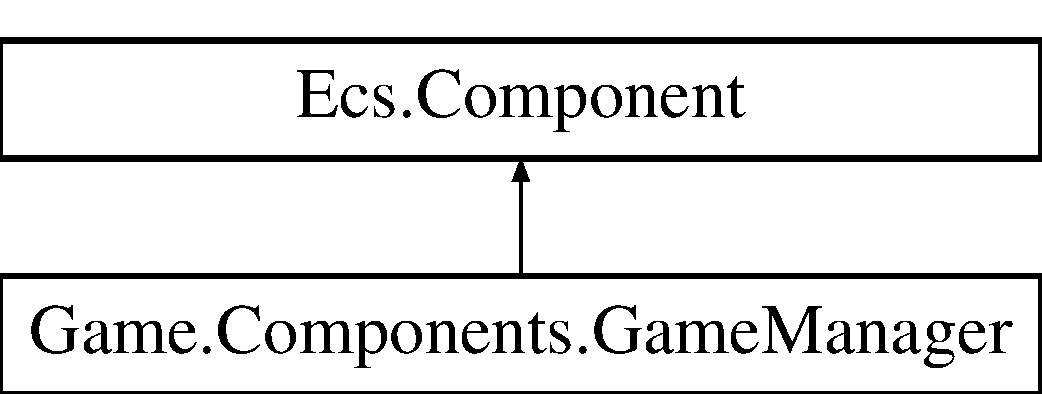
\includegraphics[height=2.000000cm]{class_game_1_1_components_1_1_game_manager}
\end{center}
\end{figure}
\subsection*{Public Member Functions}
\begin{DoxyCompactItemize}
\item 
\mbox{\Hypertarget{class_game_1_1_components_1_1_game_manager_a9bdaeb985404b402bc84f9611ecdefa7}\label{class_game_1_1_components_1_1_game_manager_a9bdaeb985404b402bc84f9611ecdefa7}} 
{\bfseries Game\+Manager} (int width, int height)
\item 
\mbox{\Hypertarget{class_game_1_1_components_1_1_game_manager_a3ad0b62c9ca08a624d841a61bb6ab1a1}\label{class_game_1_1_components_1_1_game_manager_a3ad0b62c9ca08a624d841a61bb6ab1a1}} 
override void {\bfseries Start} ()
\item 
\mbox{\Hypertarget{class_game_1_1_components_1_1_game_manager_a8b7bb5ae416225ca1232af92de3b0284}\label{class_game_1_1_components_1_1_game_manager_a8b7bb5ae416225ca1232af92de3b0284}} 
override void {\bfseries Update} ()
\item 
\mbox{\Hypertarget{class_game_1_1_components_1_1_game_manager_a366f9a3a0d77d2c483cef176eb573dfd}\label{class_game_1_1_components_1_1_game_manager_a366f9a3a0d77d2c483cef176eb573dfd}} 
override void {\bfseries Late\+Update} ()
\item 
\mbox{\Hypertarget{class_game_1_1_components_1_1_game_manager_a1bfad82d8aff8d0811fbcd93c0cc491e}\label{class_game_1_1_components_1_1_game_manager_a1bfad82d8aff8d0811fbcd93c0cc491e}} 
override void {\bfseries Render} ()
\end{DoxyCompactItemize}
\subsection*{Public Attributes}
\begin{DoxyCompactItemize}
\item 
\mbox{\Hypertarget{class_game_1_1_components_1_1_game_manager_aa50485c43a602320a7aaee3e86598d79}\label{class_game_1_1_components_1_1_game_manager_aa50485c43a602320a7aaee3e86598d79}} 
int {\bfseries game\+Width}
\item 
\mbox{\Hypertarget{class_game_1_1_components_1_1_game_manager_a3d0f30ace8ce5fdaee138e3bdb43287c}\label{class_game_1_1_components_1_1_game_manager_a3d0f30ace8ce5fdaee138e3bdb43287c}} 
int {\bfseries game\+Height}
\end{DoxyCompactItemize}


The documentation for this class was generated from the following file\+:\begin{DoxyCompactItemize}
\item 
src/\+Game/\+Components/Game\+Manager.\+cs\end{DoxyCompactItemize}

\hypertarget{class_ecs_1_1_game_object}{}\section{Ecs.\+Game\+Object Class Reference}
\label{class_ecs_1_1_game_object}\index{Ecs.\+Game\+Object@{Ecs.\+Game\+Object}}
\subsection*{Public Member Functions}
\begin{DoxyCompactItemize}
\item 
bool \mbox{\hyperlink{class_ecs_1_1_game_object_aa6bc70dfeda488ed71b536346d29881b}{Is\+Active}} ()
\begin{DoxyCompactList}\small\item\em Determines if this \mbox{\hyperlink{class_ecs_1_1_game_object}{Game\+Object}} is active in the game. \end{DoxyCompactList}\item 
void \mbox{\hyperlink{class_ecs_1_1_game_object_af4211e4cb1df45aa6692a5c2de79ef53}{Set\+Active}} (bool active)
\begin{DoxyCompactList}\small\item\em Changes this \end{DoxyCompactList}\item 
\mbox{\Hypertarget{class_ecs_1_1_game_object_a57d652307d98be5d8f4eb4c16822eed1}\label{class_ecs_1_1_game_object_a57d652307d98be5d8f4eb4c16822eed1}} 
String {\bfseries Tag} ()
\item 
\mbox{\Hypertarget{class_ecs_1_1_game_object_a075b833b0ea4e8b58cab5d2a27d9a111}\label{class_ecs_1_1_game_object_a075b833b0ea4e8b58cab5d2a27d9a111}} 
void {\bfseries Start} ()
\item 
\mbox{\Hypertarget{class_ecs_1_1_game_object_aafeda353872b30727e1394075481beff}\label{class_ecs_1_1_game_object_aafeda353872b30727e1394075481beff}} 
void {\bfseries Update} ()
\item 
\mbox{\Hypertarget{class_ecs_1_1_game_object_ad707ec0ef27791d2049a0125407539b0}\label{class_ecs_1_1_game_object_ad707ec0ef27791d2049a0125407539b0}} 
void {\bfseries Late\+Update} ()
\item 
\mbox{\Hypertarget{class_ecs_1_1_game_object_aebb472921ec1b79b8dce1a5481861746}\label{class_ecs_1_1_game_object_aebb472921ec1b79b8dce1a5481861746}} 
void {\bfseries Render} ()
\item 
\mbox{\Hypertarget{class_ecs_1_1_game_object_ab3961ec9815e23fc328c762e0f332394}\label{class_ecs_1_1_game_object_ab3961ec9815e23fc328c762e0f332394}} 
\mbox{\hyperlink{class_ecs_1_1_component}{Component}} {\bfseries Get\+Component\+In\+Children$<$ T $>$} ()
\item 
\mbox{\Hypertarget{class_ecs_1_1_game_object_abd178dde2e08b0f148ea06907a0b1302}\label{class_ecs_1_1_game_object_abd178dde2e08b0f148ea06907a0b1302}} 
\mbox{\hyperlink{class_ecs_1_1_component}{Component}} {\bfseries Add\+Component} (\mbox{\hyperlink{class_ecs_1_1_component}{Component}} component)
\item 
\mbox{\Hypertarget{class_ecs_1_1_game_object_a4d12d7a0f391cb4aa44626df35e9882f}\label{class_ecs_1_1_game_object_a4d12d7a0f391cb4aa44626df35e9882f}} 
\mbox{\hyperlink{class_ecs_1_1_component}{Component}} {\bfseries Add\+Component$<$ T $>$} ()
\item 
\mbox{\Hypertarget{class_ecs_1_1_game_object_a4263f0a68ee23088b4a7f90a7c24a22a}\label{class_ecs_1_1_game_object_a4263f0a68ee23088b4a7f90a7c24a22a}} 
\mbox{\hyperlink{class_ecs_1_1_component}{Component}} {\bfseries Get\+Component} (Type type)
\item 
\mbox{\Hypertarget{class_ecs_1_1_game_object_a46994a68c1d374811e04fa655b004102}\label{class_ecs_1_1_game_object_a46994a68c1d374811e04fa655b004102}} 
\mbox{\hyperlink{class_ecs_1_1_component}{Component}} {\bfseries Get\+Component$<$ T $>$} ()
\item 
\mbox{\Hypertarget{class_ecs_1_1_game_object_a7387d9144b92e309ea77f56760bfb31c}\label{class_ecs_1_1_game_object_a7387d9144b92e309ea77f56760bfb31c}} 
List$<$ T $>$ {\bfseries Get\+Components$<$ T $>$} ()
\item 
\mbox{\Hypertarget{class_ecs_1_1_game_object_a15d93c3cdc874773daf66282c6e55f8c}\label{class_ecs_1_1_game_object_a15d93c3cdc874773daf66282c6e55f8c}} 
int {\bfseries Instance\+ID} ()
\item 
\mbox{\Hypertarget{class_ecs_1_1_game_object_a79994c0a1e6d1b03f9ef48eeb1803385}\label{class_ecs_1_1_game_object_a79994c0a1e6d1b03f9ef48eeb1803385}} 
void {\bfseries Remove\+Component} (Type type)
\end{DoxyCompactItemize}
\subsection*{Static Public Member Functions}
\begin{DoxyCompactItemize}
\item 
\mbox{\Hypertarget{class_ecs_1_1_game_object_ae4dc7a9531fd8fa3d087b26042866fa5}\label{class_ecs_1_1_game_object_ae4dc7a9531fd8fa3d087b26042866fa5}} 
static \mbox{\hyperlink{class_ecs_1_1_game_object}{Game\+Object}} {\bfseries Instantiate} ()
\item 
\mbox{\Hypertarget{class_ecs_1_1_game_object_a88f74329a483cac3ed276a3d6f896256}\label{class_ecs_1_1_game_object_a88f74329a483cac3ed276a3d6f896256}} 
static \mbox{\hyperlink{class_ecs_1_1_game_object}{Game\+Object}} {\bfseries Instantiate} (String tag)
\item 
\mbox{\Hypertarget{class_ecs_1_1_game_object_a81390ec2e672a710e43116eb3d41df7b}\label{class_ecs_1_1_game_object_a81390ec2e672a710e43116eb3d41df7b}} 
static void {\bfseries Destroy} (\mbox{\hyperlink{class_ecs_1_1_game_object}{Game\+Object}} go)
\item 
\mbox{\Hypertarget{class_ecs_1_1_game_object_afdc4e1a061dc8dfbaa7399a86532a0da}\label{class_ecs_1_1_game_object_afdc4e1a061dc8dfbaa7399a86532a0da}} 
static \mbox{\hyperlink{class_ecs_1_1_game_object}{Game\+Object}} {\bfseries Find\+With\+Tag} (String tag)
\item 
\mbox{\Hypertarget{class_ecs_1_1_game_object_a1eb8dc519b642587b6517cb4ad569fc1}\label{class_ecs_1_1_game_object_a1eb8dc519b642587b6517cb4ad569fc1}} 
static List$<$ \mbox{\hyperlink{class_ecs_1_1_game_object}{Game\+Object}} $>$ {\bfseries Find\+Game\+Objects\+With\+Tag} (String tag)
\item 
\mbox{\Hypertarget{class_ecs_1_1_game_object_a2f4b7b28652651d02135919e75c5ad0d}\label{class_ecs_1_1_game_object_a2f4b7b28652651d02135919e75c5ad0d}} 
static Dictionary$<$ int, \mbox{\hyperlink{class_ecs_1_1_game_object}{Game\+Object}} $>$ {\bfseries Get\+Game\+Objects} ()
\end{DoxyCompactItemize}
\subsection*{Public Attributes}
\begin{DoxyCompactItemize}
\item 
\mbox{\Hypertarget{class_ecs_1_1_game_object_a0e1caafb0f43cf8d35d10e7e3b82cbb7}\label{class_ecs_1_1_game_object_a0e1caafb0f43cf8d35d10e7e3b82cbb7}} 
\mbox{\hyperlink{class_ecs_1_1_transform}{Transform}} {\bfseries transform}
\end{DoxyCompactItemize}


\subsection{Member Function Documentation}
\mbox{\Hypertarget{class_ecs_1_1_game_object_aa6bc70dfeda488ed71b536346d29881b}\label{class_ecs_1_1_game_object_aa6bc70dfeda488ed71b536346d29881b}} 
\index{Ecs\+::\+Game\+Object@{Ecs\+::\+Game\+Object}!Is\+Active@{Is\+Active}}
\index{Is\+Active@{Is\+Active}!Ecs\+::\+Game\+Object@{Ecs\+::\+Game\+Object}}
\subsubsection{\texorpdfstring{Is\+Active()}{IsActive()}}
{\footnotesize\ttfamily bool Ecs.\+Game\+Object.\+Is\+Active (\begin{DoxyParamCaption}{ }\end{DoxyParamCaption})}



Determines if this \mbox{\hyperlink{class_ecs_1_1_game_object}{Game\+Object}} is active in the game. 

\begin{DoxyReturn}{Returns}

\end{DoxyReturn}
\mbox{\Hypertarget{class_ecs_1_1_game_object_af4211e4cb1df45aa6692a5c2de79ef53}\label{class_ecs_1_1_game_object_af4211e4cb1df45aa6692a5c2de79ef53}} 
\index{Ecs\+::\+Game\+Object@{Ecs\+::\+Game\+Object}!Set\+Active@{Set\+Active}}
\index{Set\+Active@{Set\+Active}!Ecs\+::\+Game\+Object@{Ecs\+::\+Game\+Object}}
\subsubsection{\texorpdfstring{Set\+Active()}{SetActive()}}
{\footnotesize\ttfamily void Ecs.\+Game\+Object.\+Set\+Active (\begin{DoxyParamCaption}\item[{bool}]{active }\end{DoxyParamCaption})}



Changes this 

{\ttfamily \mbox{\hyperlink{class_ecs_1_1_game_object}{Game\+Object}}\textquotesingle{}s} active state. 

/// 
\begin{DoxyParams}{Parameters}
{\em active} & The true/false state to change this \mbox{\hyperlink{class_ecs_1_1_game_object}{Game\+Object}} to\\
\hline
\end{DoxyParams}



\begin{DoxyCode}
GameObject go = GameObject.Instantiate();
go.SetActive(\textcolor{keyword}{false})
\end{DoxyCode}
 

The documentation for this class was generated from the following file\+:\begin{DoxyCompactItemize}
\item 
src/\+Ecs/Game\+Object.\+cs\end{DoxyCompactItemize}

\hypertarget{class_game_1_1_components_1_1_h_u_d}{}\section{Game.\+Components.\+H\+UD Class Reference}
\label{class_game_1_1_components_1_1_h_u_d}\index{Game.\+Components.\+H\+UD@{Game.\+Components.\+H\+UD}}
Inheritance diagram for Game.\+Components.\+H\+UD\+:\begin{figure}[H]
\begin{center}
\leavevmode
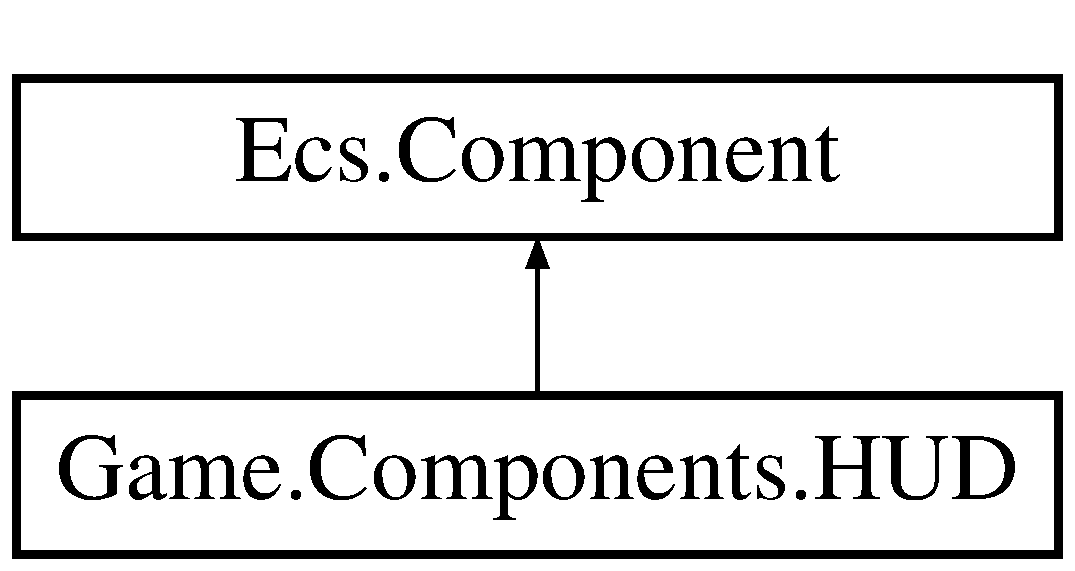
\includegraphics[height=2.000000cm]{class_game_1_1_components_1_1_h_u_d}
\end{center}
\end{figure}
\subsection*{Public Member Functions}
\begin{DoxyCompactItemize}
\item 
\mbox{\Hypertarget{class_game_1_1_components_1_1_h_u_d_aea9e5880d4b970eba116f1655a4e3b16}\label{class_game_1_1_components_1_1_h_u_d_aea9e5880d4b970eba116f1655a4e3b16}} 
{\bfseries H\+UD} (int width, int height)
\item 
\mbox{\Hypertarget{class_game_1_1_components_1_1_h_u_d_aca74740e211eeca07cd6ed4b6dde7b8d}\label{class_game_1_1_components_1_1_h_u_d_aca74740e211eeca07cd6ed4b6dde7b8d}} 
void {\bfseries Log} (String line)
\item 
\mbox{\Hypertarget{class_game_1_1_components_1_1_h_u_d_a214dfb53aba288d958d1f4a565155aba}\label{class_game_1_1_components_1_1_h_u_d_a214dfb53aba288d958d1f4a565155aba}} 
override void {\bfseries Start} ()
\item 
\mbox{\Hypertarget{class_game_1_1_components_1_1_h_u_d_a018dd412d1e5a6650b0dddb68e0da051}\label{class_game_1_1_components_1_1_h_u_d_a018dd412d1e5a6650b0dddb68e0da051}} 
override void {\bfseries Update} ()
\item 
\mbox{\Hypertarget{class_game_1_1_components_1_1_h_u_d_ab3f42934b91fd4c72caef545a8b6d9f6}\label{class_game_1_1_components_1_1_h_u_d_ab3f42934b91fd4c72caef545a8b6d9f6}} 
override void {\bfseries Render} ()
\end{DoxyCompactItemize}
\subsection*{Additional Inherited Members}


The documentation for this class was generated from the following file\+:\begin{DoxyCompactItemize}
\item 
src/\+Game/\+Components/H\+U\+D.\+cs\end{DoxyCompactItemize}

\hypertarget{interface_game_1_1_interfaces_1_1_i_damageable}{}\section{Game.\+Interfaces.\+I\+Damageable Interface Reference}
\label{interface_game_1_1_interfaces_1_1_i_damageable}\index{Game.\+Interfaces.\+I\+Damageable@{Game.\+Interfaces.\+I\+Damageable}}
Inheritance diagram for Game.\+Interfaces.\+I\+Damageable\+:\begin{figure}[H]
\begin{center}
\leavevmode
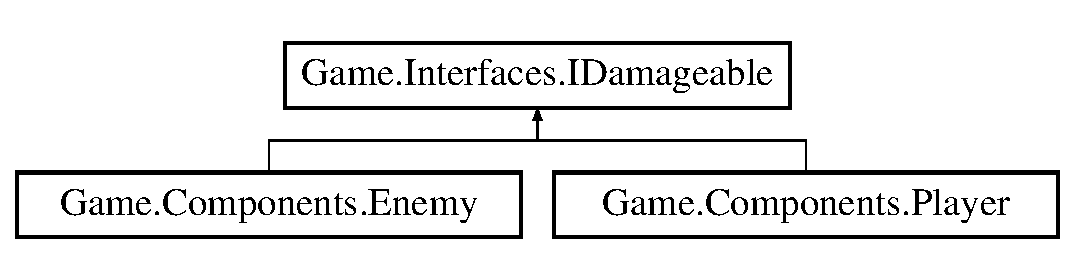
\includegraphics[height=2.000000cm]{interface_game_1_1_interfaces_1_1_i_damageable}
\end{center}
\end{figure}
\subsection*{Public Member Functions}
\begin{DoxyCompactItemize}
\item 
\mbox{\Hypertarget{interface_game_1_1_interfaces_1_1_i_damageable_a29371d7fde6f0536946a48ca48ea82c4}\label{interface_game_1_1_interfaces_1_1_i_damageable_a29371d7fde6f0536946a48ca48ea82c4}} 
void {\bfseries Apply\+Damage} (int damage)
\item 
\mbox{\Hypertarget{interface_game_1_1_interfaces_1_1_i_damageable_a6df7fc5928a7ecad3ea5bf323d98cf00}\label{interface_game_1_1_interfaces_1_1_i_damageable_a6df7fc5928a7ecad3ea5bf323d98cf00}} 
void {\bfseries On\+Death} ()
\end{DoxyCompactItemize}


The documentation for this interface was generated from the following file\+:\begin{DoxyCompactItemize}
\item 
src/\+Game/\+Interfaces/I\+Damageable.\+cs\end{DoxyCompactItemize}

\hypertarget{interface_game_1_1_interfaces_1_1_i_movable}{}\section{Game.\+Interfaces.\+I\+Movable Interface Reference}
\label{interface_game_1_1_interfaces_1_1_i_movable}\index{Game.\+Interfaces.\+I\+Movable@{Game.\+Interfaces.\+I\+Movable}}
Inheritance diagram for Game.\+Interfaces.\+I\+Movable\+:\begin{figure}[H]
\begin{center}
\leavevmode
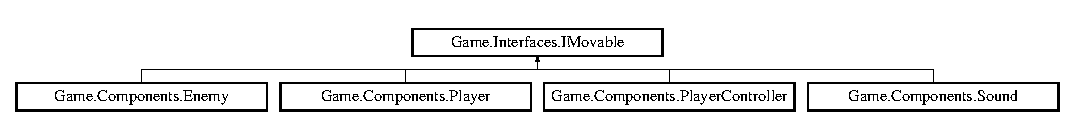
\includegraphics[height=1.261261cm]{interface_game_1_1_interfaces_1_1_i_movable}
\end{center}
\end{figure}
\subsection*{Public Member Functions}
\begin{DoxyCompactItemize}
\item 
\mbox{\Hypertarget{interface_game_1_1_interfaces_1_1_i_movable_ae34f2a106867e1ff366086748c8dea7a}\label{interface_game_1_1_interfaces_1_1_i_movable_ae34f2a106867e1ff366086748c8dea7a}} 
void {\bfseries Move} (int dx, int dy)
\end{DoxyCompactItemize}


The documentation for this interface was generated from the following file\+:\begin{DoxyCompactItemize}
\item 
src/\+Game/\+Interfaces/I\+Movable.\+cs\end{DoxyCompactItemize}

\hypertarget{class_i_o_1_1_input}{}\section{I\+O.\+Input Class Reference}
\label{class_i_o_1_1_input}\index{I\+O.\+Input@{I\+O.\+Input}}
\subsection*{Static Public Member Functions}
\begin{DoxyCompactItemize}
\item 
\mbox{\Hypertarget{class_i_o_1_1_input_a68bf573955c7c1159fd3ccacd6edc921}\label{class_i_o_1_1_input_a68bf573955c7c1159fd3ccacd6edc921}} 
static Console\+Key\+Info {\bfseries Read\+Key} ()
\item 
\mbox{\Hypertarget{class_i_o_1_1_input_adb31cb049fb35e721a26c96172c8da72}\label{class_i_o_1_1_input_adb31cb049fb35e721a26c96172c8da72}} 
static bool {\bfseries Any\+Key} ()
\item 
\mbox{\Hypertarget{class_i_o_1_1_input_a5e6c5e82708cc1f2a0a7b31897660fff}\label{class_i_o_1_1_input_a5e6c5e82708cc1f2a0a7b31897660fff}} 
static void {\bfseries Reset} ()
\end{DoxyCompactItemize}


The documentation for this class was generated from the following file\+:\begin{DoxyCompactItemize}
\item 
src/\+I\+O/Input.\+cs\end{DoxyCompactItemize}

\hypertarget{class_game_1_1_components_1_1_map}{}\section{Game.\+Components.\+Map Class Reference}
\label{class_game_1_1_components_1_1_map}\index{Game.\+Components.\+Map@{Game.\+Components.\+Map}}
Inheritance diagram for Game.\+Components.\+Map\+:\begin{figure}[H]
\begin{center}
\leavevmode
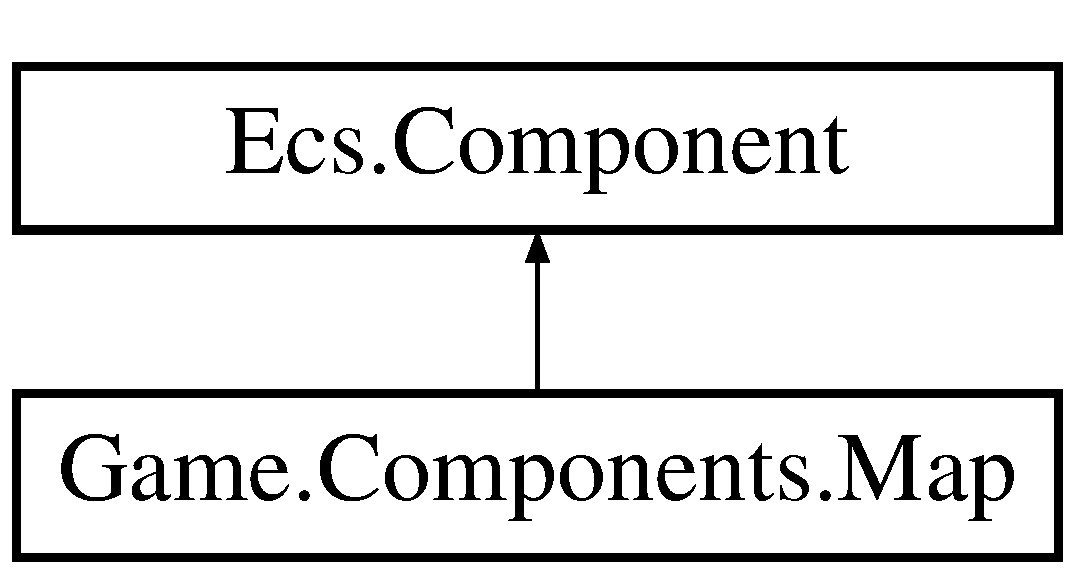
\includegraphics[height=2.000000cm]{class_game_1_1_components_1_1_map}
\end{center}
\end{figure}
\subsection*{Public Member Functions}
\begin{DoxyCompactItemize}
\item 
\mbox{\Hypertarget{class_game_1_1_components_1_1_map_a8122de6273464b91b3cde875c9ba7e15}\label{class_game_1_1_components_1_1_map_a8122de6273464b91b3cde875c9ba7e15}} 
{\bfseries Map} (int width, int height)
\item 
\mbox{\Hypertarget{class_game_1_1_components_1_1_map_a9bb57937d513bfae5fb51a1477ef8456}\label{class_game_1_1_components_1_1_map_a9bb57937d513bfae5fb51a1477ef8456}} 
override void {\bfseries Start} ()
\item 
\mbox{\Hypertarget{class_game_1_1_components_1_1_map_a23340727d22afd422ed047a0d0d1e184}\label{class_game_1_1_components_1_1_map_a23340727d22afd422ed047a0d0d1e184}} 
override void {\bfseries Update} ()
\item 
\mbox{\Hypertarget{class_game_1_1_components_1_1_map_afc6ca1cbba37b885fecc747f1d3a51c8}\label{class_game_1_1_components_1_1_map_afc6ca1cbba37b885fecc747f1d3a51c8}} 
override void {\bfseries Render} ()
\item 
\mbox{\Hypertarget{class_game_1_1_components_1_1_map_a0a50acd39192416888cf43d2f0d513b2}\label{class_game_1_1_components_1_1_map_a0a50acd39192416888cf43d2f0d513b2}} 
\mbox{\hyperlink{namespace_game_1_1_data_structures_a24fec17346a5ad535ffe81e59a617f57}{Cell\+State}} {\bfseries Get\+Cell\+State} (int x, int y)
\item 
\mbox{\Hypertarget{class_game_1_1_components_1_1_map_a10b22835af2f71512386eab23b5027cb}\label{class_game_1_1_components_1_1_map_a10b22835af2f71512386eab23b5027cb}} 
\mbox{\hyperlink{class_ecs_1_1_game_object}{Game\+Object}} {\bfseries Peek\+Object} (int x, int y)
\item 
\mbox{\Hypertarget{class_game_1_1_components_1_1_map_ad1294a28a4ebcad1087c7a29484e31e6}\label{class_game_1_1_components_1_1_map_ad1294a28a4ebcad1087c7a29484e31e6}} 
\mbox{\hyperlink{class_ecs_1_1_game_object}{Game\+Object}} {\bfseries Pop\+Object} (int x, int y)
\end{DoxyCompactItemize}
\subsection*{Public Attributes}
\begin{DoxyCompactItemize}
\item 
\mbox{\Hypertarget{class_game_1_1_components_1_1_map_a296f59890d41bd1f17d5acd56bcb834d}\label{class_game_1_1_components_1_1_map_a296f59890d41bd1f17d5acd56bcb834d}} 
int {\bfseries startingX} = 0
\item 
\mbox{\Hypertarget{class_game_1_1_components_1_1_map_ace517f9735e18d693259f6dc5ff465b0}\label{class_game_1_1_components_1_1_map_ace517f9735e18d693259f6dc5ff465b0}} 
int {\bfseries startingY} = 0
\end{DoxyCompactItemize}


The documentation for this class was generated from the following file\+:\begin{DoxyCompactItemize}
\item 
src/\+Game/\+Components/Map.\+cs\end{DoxyCompactItemize}

\hypertarget{class_game_1_1_components_1_1_model}{}\section{Game.\+Components.\+Model Class Reference}
\label{class_game_1_1_components_1_1_model}\index{Game.\+Components.\+Model@{Game.\+Components.\+Model}}
Inheritance diagram for Game.\+Components.\+Model\+:\begin{figure}[H]
\begin{center}
\leavevmode
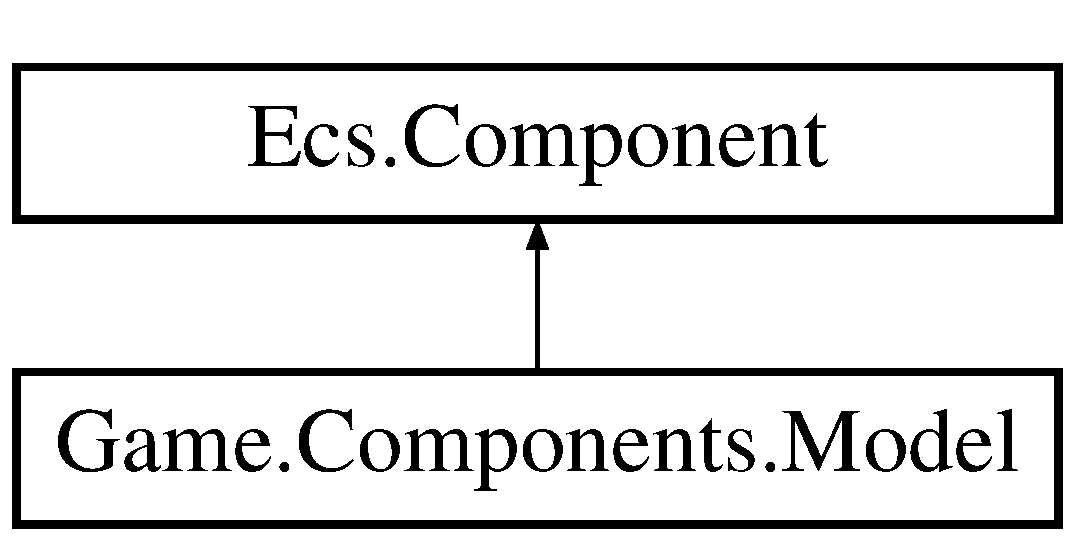
\includegraphics[height=2.000000cm]{class_game_1_1_components_1_1_model}
\end{center}
\end{figure}
\subsection*{Public Member Functions}
\begin{DoxyCompactItemize}
\item 
\mbox{\Hypertarget{class_game_1_1_components_1_1_model_ae7438c8378351cf33450728c6410d49d}\label{class_game_1_1_components_1_1_model_ae7438c8378351cf33450728c6410d49d}} 
override void {\bfseries Start} ()
\item 
\mbox{\Hypertarget{class_game_1_1_components_1_1_model_abb361907f4eb9412f9b95f6e81526832}\label{class_game_1_1_components_1_1_model_abb361907f4eb9412f9b95f6e81526832}} 
override void {\bfseries Update} ()
\item 
\mbox{\Hypertarget{class_game_1_1_components_1_1_model_aba4beeaf23138d25c8f855c2c067348c}\label{class_game_1_1_components_1_1_model_aba4beeaf23138d25c8f855c2c067348c}} 
override void {\bfseries Render} ()
\end{DoxyCompactItemize}
\subsection*{Public Attributes}
\begin{DoxyCompactItemize}
\item 
\mbox{\Hypertarget{class_game_1_1_components_1_1_model_a66f6200b14429fe5de4b34dc89af8251}\label{class_game_1_1_components_1_1_model_a66f6200b14429fe5de4b34dc89af8251}} 
List$<$ String $>$ {\bfseries model} = new List$<$String$>$()
\item 
\mbox{\Hypertarget{class_game_1_1_components_1_1_model_ad071eb5b01d238c9ae002ffc6a945d87}\label{class_game_1_1_components_1_1_model_ad071eb5b01d238c9ae002ffc6a945d87}} 
List$<$ List$<$ String $>$ $>$ {\bfseries color\+Model} = new List$<$List$<$String$>$$>$()
\end{DoxyCompactItemize}


The documentation for this class was generated from the following file\+:\begin{DoxyCompactItemize}
\item 
src/\+Game/\+Components/Model.\+cs\end{DoxyCompactItemize}

\hypertarget{class_game_1_1_data_1_1_monster_generator}{}\section{Game.\+Data.\+Monster\+Generator Class Reference}
\label{class_game_1_1_data_1_1_monster_generator}\index{Game.\+Data.\+Monster\+Generator@{Game.\+Data.\+Monster\+Generator}}
\subsection*{Static Public Member Functions}
\begin{DoxyCompactItemize}
\item 
static void \mbox{\hyperlink{class_game_1_1_data_1_1_monster_generator_af19d4d4af73485500bf648541c0a732b}{Fill}} (Random rand, int level, \mbox{\hyperlink{class_ecs_1_1_game_object}{Game\+Object}} slot)
\begin{DoxyCompactList}\small\item\em This function takes in a reference to the Random class, a level, and a Game\+Object and randomly selects a monster and generates the enemy. \end{DoxyCompactList}\end{DoxyCompactItemize}


\subsection{Member Function Documentation}
\mbox{\Hypertarget{class_game_1_1_data_1_1_monster_generator_af19d4d4af73485500bf648541c0a732b}\label{class_game_1_1_data_1_1_monster_generator_af19d4d4af73485500bf648541c0a732b}} 
\index{Game\+::\+Data\+::\+Monster\+Generator@{Game\+::\+Data\+::\+Monster\+Generator}!Fill@{Fill}}
\index{Fill@{Fill}!Game\+::\+Data\+::\+Monster\+Generator@{Game\+::\+Data\+::\+Monster\+Generator}}
\subsubsection{\texorpdfstring{Fill()}{Fill()}}
{\footnotesize\ttfamily static void Game.\+Data.\+Monster\+Generator.\+Fill (\begin{DoxyParamCaption}\item[{Random}]{rand,  }\item[{int}]{level,  }\item[{\mbox{\hyperlink{class_ecs_1_1_game_object}{Game\+Object}}}]{slot }\end{DoxyParamCaption})\hspace{0.3cm}{\ttfamily [static]}}



This function takes in a reference to the Random class, a level, and a Game\+Object and randomly selects a monster and generates the enemy. 


\begin{DoxyParams}{Parameters}
{\em rand} & \\
\hline
{\em level} & \\
\hline
{\em slot} & \\
\hline
\end{DoxyParams}


The documentation for this class was generated from the following file\+:\begin{DoxyCompactItemize}
\item 
src/\+Game/\+Data/Monster\+Generator.\+cs\end{DoxyCompactItemize}

\hypertarget{class_game_1_1_components_1_1_player}{}\section{Game.\+Components.\+Player Class Reference}
\label{class_game_1_1_components_1_1_player}\index{Game.\+Components.\+Player@{Game.\+Components.\+Player}}
Inheritance diagram for Game.\+Components.\+Player\+:\begin{figure}[H]
\begin{center}
\leavevmode
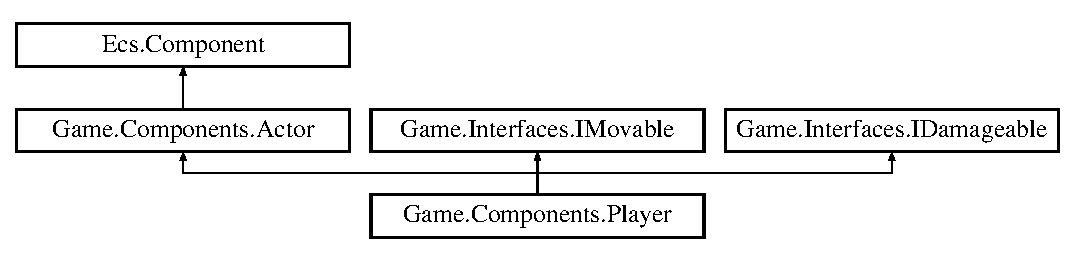
\includegraphics[height=2.962963cm]{class_game_1_1_components_1_1_player}
\end{center}
\end{figure}
\subsection*{Public Member Functions}
\begin{DoxyCompactItemize}
\item 
\mbox{\Hypertarget{class_game_1_1_components_1_1_player_ae996f7b3c2a6434e07ddb7bba59fb8cc}\label{class_game_1_1_components_1_1_player_ae996f7b3c2a6434e07ddb7bba59fb8cc}} 
override void {\bfseries Start} ()
\item 
\mbox{\Hypertarget{class_game_1_1_components_1_1_player_afdf089af59c27adb11135a2aa0bd6d82}\label{class_game_1_1_components_1_1_player_afdf089af59c27adb11135a2aa0bd6d82}} 
override void {\bfseries Update} ()
\item 
\mbox{\Hypertarget{class_game_1_1_components_1_1_player_a7b96fcfa280c3d04459ca4d3bfe27f64}\label{class_game_1_1_components_1_1_player_a7b96fcfa280c3d04459ca4d3bfe27f64}} 
override void {\bfseries Render} ()
\item 
\mbox{\Hypertarget{class_game_1_1_components_1_1_player_a42ef5b1e74faa75f955758eb83a45ed4}\label{class_game_1_1_components_1_1_player_a42ef5b1e74faa75f955758eb83a45ed4}} 
override void {\bfseries On\+Enable} ()
\item 
\mbox{\Hypertarget{class_game_1_1_components_1_1_player_a77dcd93c47d77201b83eefcb1bc79104}\label{class_game_1_1_components_1_1_player_a77dcd93c47d77201b83eefcb1bc79104}} 
override void {\bfseries On\+Disable} ()
\item 
\mbox{\Hypertarget{class_game_1_1_components_1_1_player_a224dce2f4af9381dcd34d3f91571b8e3}\label{class_game_1_1_components_1_1_player_a224dce2f4af9381dcd34d3f91571b8e3}} 
void {\bfseries Move} (int dx, int dy)
\item 
\mbox{\Hypertarget{class_game_1_1_components_1_1_player_acfecb95f166bf3cb0c6906491d602b5a}\label{class_game_1_1_components_1_1_player_acfecb95f166bf3cb0c6906491d602b5a}} 
void {\bfseries Apply\+Damage} (int damage)
\item 
\mbox{\Hypertarget{class_game_1_1_components_1_1_player_a267d9db6071a2aa43becb5b200de6bb5}\label{class_game_1_1_components_1_1_player_a267d9db6071a2aa43becb5b200de6bb5}} 
void {\bfseries On\+Death} ()
\end{DoxyCompactItemize}
\subsection*{Additional Inherited Members}


The documentation for this class was generated from the following file\+:\begin{DoxyCompactItemize}
\item 
src/\+Game/\+Components/Player.\+cs\end{DoxyCompactItemize}

\hypertarget{class_game_1_1_components_1_1_player_controller}{}\section{Game.\+Components.\+Player\+Controller Class Reference}
\label{class_game_1_1_components_1_1_player_controller}\index{Game.\+Components.\+Player\+Controller@{Game.\+Components.\+Player\+Controller}}
Inheritance diagram for Game.\+Components.\+Player\+Controller\+:\begin{figure}[H]
\begin{center}
\leavevmode
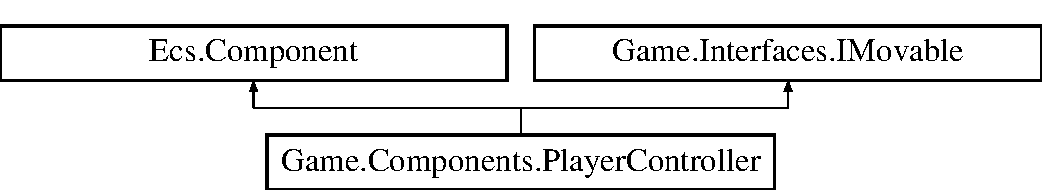
\includegraphics[height=2.000000cm]{class_game_1_1_components_1_1_player_controller}
\end{center}
\end{figure}
\subsection*{Public Member Functions}
\begin{DoxyCompactItemize}
\item 
\mbox{\Hypertarget{class_game_1_1_components_1_1_player_controller_ab119c5a22d67c566424afc1e6078821a}\label{class_game_1_1_components_1_1_player_controller_ab119c5a22d67c566424afc1e6078821a}} 
override void {\bfseries Start} ()
\item 
\mbox{\Hypertarget{class_game_1_1_components_1_1_player_controller_ad2c959b663b69b669c274636a813fc80}\label{class_game_1_1_components_1_1_player_controller_ad2c959b663b69b669c274636a813fc80}} 
override void {\bfseries On\+Enable} ()
\item 
\mbox{\Hypertarget{class_game_1_1_components_1_1_player_controller_aa31b1af2002d8c806ccb39651bb591cd}\label{class_game_1_1_components_1_1_player_controller_aa31b1af2002d8c806ccb39651bb591cd}} 
override void {\bfseries Update} ()
\item 
\mbox{\Hypertarget{class_game_1_1_components_1_1_player_controller_ae6fe9aee3cee653cfe3385c0049dd044}\label{class_game_1_1_components_1_1_player_controller_ae6fe9aee3cee653cfe3385c0049dd044}} 
override void {\bfseries Render} ()
\item 
\mbox{\Hypertarget{class_game_1_1_components_1_1_player_controller_a1f1bf27d4db033b3fc45022278b8c17e}\label{class_game_1_1_components_1_1_player_controller_a1f1bf27d4db033b3fc45022278b8c17e}} 
void {\bfseries Move} (int dx, int dy)
\end{DoxyCompactItemize}
\subsection*{Additional Inherited Members}


The documentation for this class was generated from the following file\+:\begin{DoxyCompactItemize}
\item 
src/\+Game/\+Components/Player\+Controller.\+cs\end{DoxyCompactItemize}

\hypertarget{class_program}{}\section{Program Class Reference}
\label{class_program}\index{Program@{Program}}


The documentation for this class was generated from the following file\+:\begin{DoxyCompactItemize}
\item 
src/Program.\+cs\end{DoxyCompactItemize}

\hypertarget{class_game_1_1_dungeon_maker_1_1_room}{}\section{Game.\+Dungeon\+Maker.\+Room Class Reference}
\label{class_game_1_1_dungeon_maker_1_1_room}\index{Game.\+Dungeon\+Maker.\+Room@{Game.\+Dungeon\+Maker.\+Room}}
\subsection*{Public Member Functions}
\begin{DoxyCompactItemize}
\item 
\mbox{\hyperlink{class_game_1_1_dungeon_maker_1_1_room_abbd9573ede25a9fce7675034863542d9}{Room}} (int width, int height, int x, int y)
\begin{DoxyCompactList}\small\item\em Creates a {\ttfamily \mbox{\hyperlink{class_game_1_1_dungeon_maker_1_1_room}{Room}}} object with a specific width/height at a specific x/y location. \end{DoxyCompactList}\end{DoxyCompactItemize}
\subsection*{Public Attributes}
\begin{DoxyCompactItemize}
\item 
\mbox{\Hypertarget{class_game_1_1_dungeon_maker_1_1_room_a732fdc6d23d0cf6de459470b6cbc2423}\label{class_game_1_1_dungeon_maker_1_1_room_a732fdc6d23d0cf6de459470b6cbc2423}} 
int {\bfseries width}
\item 
\mbox{\Hypertarget{class_game_1_1_dungeon_maker_1_1_room_a85af9703757169cabe5b1013a986550f}\label{class_game_1_1_dungeon_maker_1_1_room_a85af9703757169cabe5b1013a986550f}} 
int {\bfseries height}
\item 
\mbox{\Hypertarget{class_game_1_1_dungeon_maker_1_1_room_a86997730f14143525d7b7006ca6c1472}\label{class_game_1_1_dungeon_maker_1_1_room_a86997730f14143525d7b7006ca6c1472}} 
int {\bfseries x}
\item 
\mbox{\Hypertarget{class_game_1_1_dungeon_maker_1_1_room_a50f07d97020c6d21362a6db20b0139b0}\label{class_game_1_1_dungeon_maker_1_1_room_a50f07d97020c6d21362a6db20b0139b0}} 
int {\bfseries y}
\end{DoxyCompactItemize}


\subsection{Constructor \& Destructor Documentation}
\mbox{\Hypertarget{class_game_1_1_dungeon_maker_1_1_room_abbd9573ede25a9fce7675034863542d9}\label{class_game_1_1_dungeon_maker_1_1_room_abbd9573ede25a9fce7675034863542d9}} 
\index{Game\+::\+Dungeon\+Maker\+::\+Room@{Game\+::\+Dungeon\+Maker\+::\+Room}!Room@{Room}}
\index{Room@{Room}!Game\+::\+Dungeon\+Maker\+::\+Room@{Game\+::\+Dungeon\+Maker\+::\+Room}}
\subsubsection{\texorpdfstring{Room()}{Room()}}
{\footnotesize\ttfamily Game.\+Dungeon\+Maker.\+Room.\+Room (\begin{DoxyParamCaption}\item[{int}]{width,  }\item[{int}]{height,  }\item[{int}]{x,  }\item[{int}]{y }\end{DoxyParamCaption})}



Creates a {\ttfamily \mbox{\hyperlink{class_game_1_1_dungeon_maker_1_1_room}{Room}}} object with a specific width/height at a specific x/y location. 


\begin{DoxyParams}{Parameters}
{\em width} & The width of the room\\
\hline
{\em height} & The height of the room\\
\hline
{\em x} & The x coordinate of the room\textquotesingle{}s top left corner\\
\hline
{\em y} & The y coordinate of the room\textquotesingle{}s top left corner\\
\hline
\end{DoxyParams}


The documentation for this class was generated from the following file\+:\begin{DoxyCompactItemize}
\item 
src/\+Game/\+Dungeon\+Maker/Room.\+cs\end{DoxyCompactItemize}

\hypertarget{class_game_1_1_components_1_1_sound}{}\section{Game.\+Components.\+Sound Class Reference}
\label{class_game_1_1_components_1_1_sound}\index{Game.\+Components.\+Sound@{Game.\+Components.\+Sound}}
Inheritance diagram for Game.\+Components.\+Sound\+:\begin{figure}[H]
\begin{center}
\leavevmode
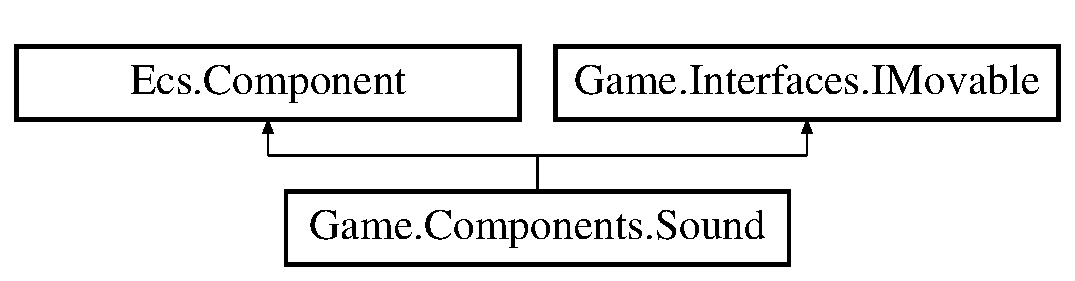
\includegraphics[height=2.000000cm]{class_game_1_1_components_1_1_sound}
\end{center}
\end{figure}
\subsection*{Public Member Functions}
\begin{DoxyCompactItemize}
\item 
\mbox{\Hypertarget{class_game_1_1_components_1_1_sound_abd2895a930b17f9f5c9be789b1e8435c}\label{class_game_1_1_components_1_1_sound_abd2895a930b17f9f5c9be789b1e8435c}} 
override void {\bfseries Start} ()
\item 
\mbox{\Hypertarget{class_game_1_1_components_1_1_sound_a814b11a6bfb40260d91e4b39f74ccd6f}\label{class_game_1_1_components_1_1_sound_a814b11a6bfb40260d91e4b39f74ccd6f}} 
override void {\bfseries Update} ()
\item 
\mbox{\Hypertarget{class_game_1_1_components_1_1_sound_afbb7ad1658564bbd716c9770b565dbe1}\label{class_game_1_1_components_1_1_sound_afbb7ad1658564bbd716c9770b565dbe1}} 
override void {\bfseries Render} ()
\item 
\mbox{\Hypertarget{class_game_1_1_components_1_1_sound_ad41d2930349a5ddc1d46955b630b19e5}\label{class_game_1_1_components_1_1_sound_ad41d2930349a5ddc1d46955b630b19e5}} 
void {\bfseries Move} (int dx, int dy)
\end{DoxyCompactItemize}
\subsection*{Additional Inherited Members}


The documentation for this class was generated from the following file\+:\begin{DoxyCompactItemize}
\item 
src/\+Game/\+Components/Sound.\+cs\end{DoxyCompactItemize}

\hypertarget{class_game_1_1_components_1_1_spawn_manager}{}\section{Game.\+Components.\+Spawn\+Manager Class Reference}
\label{class_game_1_1_components_1_1_spawn_manager}\index{Game.\+Components.\+Spawn\+Manager@{Game.\+Components.\+Spawn\+Manager}}
Inheritance diagram for Game.\+Components.\+Spawn\+Manager\+:\begin{figure}[H]
\begin{center}
\leavevmode
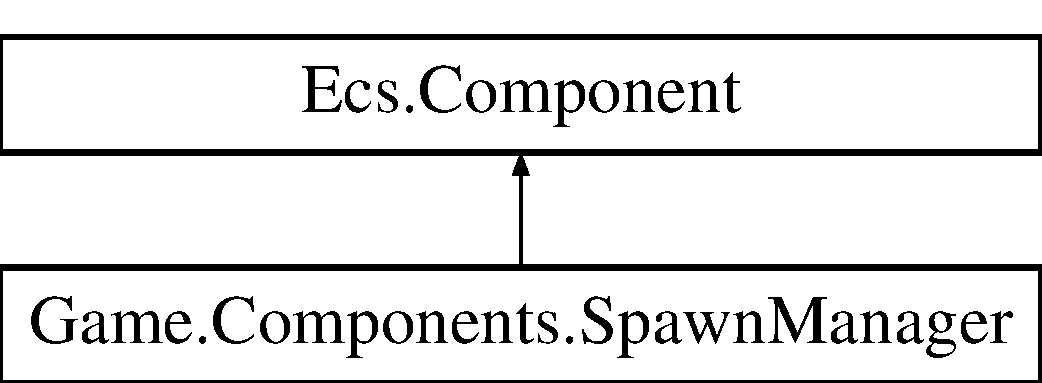
\includegraphics[height=2.000000cm]{class_game_1_1_components_1_1_spawn_manager}
\end{center}
\end{figure}
\subsection*{Public Member Functions}
\begin{DoxyCompactItemize}
\item 
\mbox{\Hypertarget{class_game_1_1_components_1_1_spawn_manager_ac81b1b98739121be3647956943ea7ccc}\label{class_game_1_1_components_1_1_spawn_manager_ac81b1b98739121be3647956943ea7ccc}} 
override void {\bfseries Start} ()
\item 
\mbox{\Hypertarget{class_game_1_1_components_1_1_spawn_manager_a86d9fad9c565c5e0adf713ced758c717}\label{class_game_1_1_components_1_1_spawn_manager_a86d9fad9c565c5e0adf713ced758c717}} 
override void {\bfseries Update} ()
\item 
\mbox{\Hypertarget{class_game_1_1_components_1_1_spawn_manager_a9e824ce8907edb4487fbb52c23065893}\label{class_game_1_1_components_1_1_spawn_manager_a9e824ce8907edb4487fbb52c23065893}} 
override void {\bfseries Render} ()
\item 
\mbox{\Hypertarget{class_game_1_1_components_1_1_spawn_manager_aa178e4c7d6952bf876d20e6c2a8e4ffd}\label{class_game_1_1_components_1_1_spawn_manager_aa178e4c7d6952bf876d20e6c2a8e4ffd}} 
\mbox{\hyperlink{class_ecs_1_1_game_object}{Game\+Object}} {\bfseries Create\+Enemy} (int x, int y, int level)
\item 
\mbox{\Hypertarget{class_game_1_1_components_1_1_spawn_manager_ab42c59bd9c39ab52046e99f876261ed2}\label{class_game_1_1_components_1_1_spawn_manager_ab42c59bd9c39ab52046e99f876261ed2}} 
\mbox{\hyperlink{class_ecs_1_1_game_object}{Game\+Object}} {\bfseries Create\+Door} (int x, int y)
\end{DoxyCompactItemize}
\subsection*{Additional Inherited Members}


The documentation for this class was generated from the following file\+:\begin{DoxyCompactItemize}
\item 
src/\+Game/\+Components/Spawn\+Manager.\+cs\end{DoxyCompactItemize}

\hypertarget{class_ecs_1_1_time}{}\section{Ecs.\+Time Class Reference}
\label{class_ecs_1_1_time}\index{Ecs.\+Time@{Ecs.\+Time}}
\subsection*{Static Public Member Functions}
\begin{DoxyCompactItemize}
\item 
\mbox{\Hypertarget{class_ecs_1_1_time_a435837193cce74947d0fc63b6f14f36f}\label{class_ecs_1_1_time_a435837193cce74947d0fc63b6f14f36f}} 
static void {\bfseries Initialize} ()
\item 
\mbox{\Hypertarget{class_ecs_1_1_time_a7d98fab0c7c708ea1f1adab0af3a7a7f}\label{class_ecs_1_1_time_a7d98fab0c7c708ea1f1adab0af3a7a7f}} 
static void {\bfseries Update} ()
\end{DoxyCompactItemize}
\subsection*{Static Public Attributes}
\begin{DoxyCompactItemize}
\item 
\mbox{\Hypertarget{class_ecs_1_1_time_a149d65fe7eb9f87c12cbd846af94578f}\label{class_ecs_1_1_time_a149d65fe7eb9f87c12cbd846af94578f}} 
static long {\bfseries delta\+Ticks} = 0
\end{DoxyCompactItemize}


The documentation for this class was generated from the following file\+:\begin{DoxyCompactItemize}
\item 
src/\+Ecs/Time.\+cs\end{DoxyCompactItemize}

\hypertarget{class_ecs_1_1_transform}{}\section{Ecs.\+Transform Class Reference}
\label{class_ecs_1_1_transform}\index{Ecs.\+Transform@{Ecs.\+Transform}}
Inheritance diagram for Ecs.\+Transform\+:\begin{figure}[H]
\begin{center}
\leavevmode
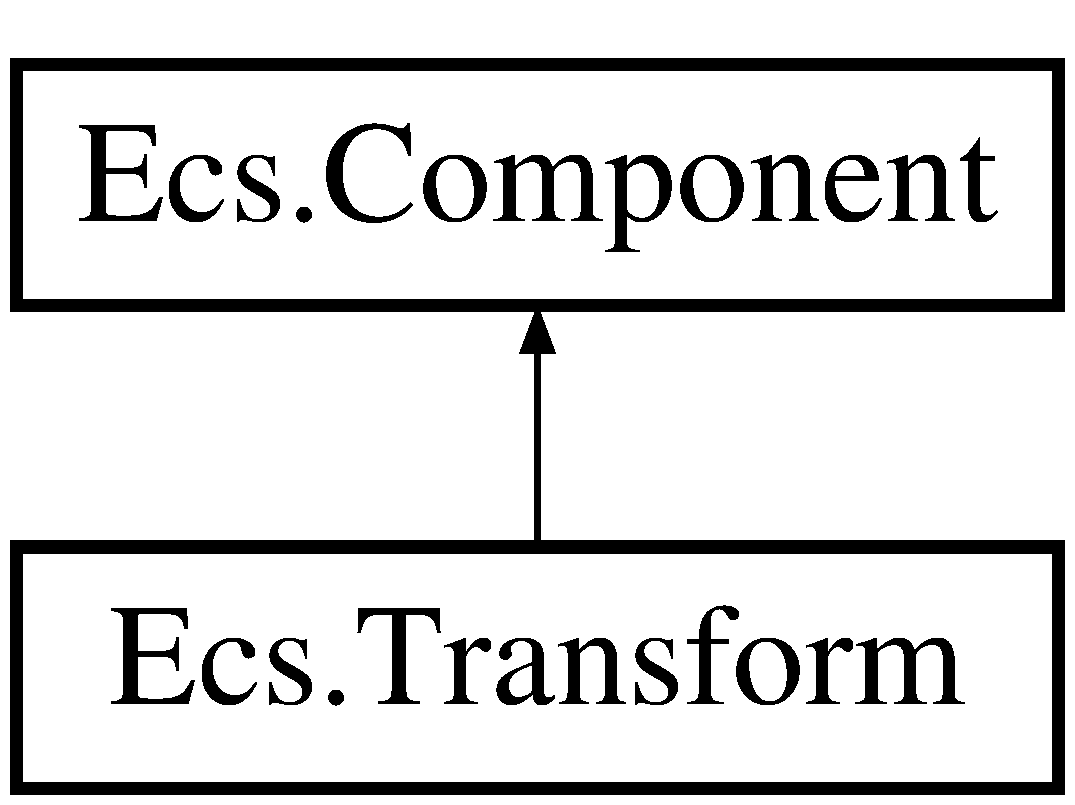
\includegraphics[height=2.000000cm]{class_ecs_1_1_transform}
\end{center}
\end{figure}
\subsection*{Public Member Functions}
\begin{DoxyCompactItemize}
\item 
\mbox{\Hypertarget{class_ecs_1_1_transform_ade54f8a35651662e0e91360effc3a052}\label{class_ecs_1_1_transform_ade54f8a35651662e0e91360effc3a052}} 
void {\bfseries Set\+Parent} (\mbox{\hyperlink{class_ecs_1_1_transform}{Transform}} transform)
\item 
\mbox{\Hypertarget{class_ecs_1_1_transform_a2f303a5ea45c21cd198f3d11ec6cfe32}\label{class_ecs_1_1_transform_a2f303a5ea45c21cd198f3d11ec6cfe32}} 
void {\bfseries Translate} (int dx, int dy)
\end{DoxyCompactItemize}
\subsection*{Public Attributes}
\begin{DoxyCompactItemize}
\item 
\mbox{\Hypertarget{class_ecs_1_1_transform_a0bfde38740639bf3e01b4a1d6029c7d6}\label{class_ecs_1_1_transform_a0bfde38740639bf3e01b4a1d6029c7d6}} 
\mbox{\hyperlink{class_ecs_1_1_transform}{Transform}} {\bfseries parent} = null
\item 
\mbox{\Hypertarget{class_ecs_1_1_transform_a0f95eb68f151048d53a81c02551764da}\label{class_ecs_1_1_transform_a0f95eb68f151048d53a81c02551764da}} 
List$<$ \mbox{\hyperlink{class_ecs_1_1_transform}{Transform}} $>$ {\bfseries children} = new List$<$\mbox{\hyperlink{class_ecs_1_1_transform}{Transform}}$>$()
\item 
\mbox{\Hypertarget{class_ecs_1_1_transform_a686a025cfea0490a5e5f43c5ba968dfc}\label{class_ecs_1_1_transform_a686a025cfea0490a5e5f43c5ba968dfc}} 
\mbox{\hyperlink{class_ecs_1_1_vec2i}{Vec2i}} {\bfseries position} = new \mbox{\hyperlink{class_ecs_1_1_vec2i}{Vec2i}}()
\end{DoxyCompactItemize}


The documentation for this class was generated from the following file\+:\begin{DoxyCompactItemize}
\item 
src/\+Ecs/Transform.\+cs\end{DoxyCompactItemize}

\hypertarget{class_ecs_1_1_vec2i}{}\section{Ecs.\+Vec2i Class Reference}
\label{class_ecs_1_1_vec2i}\index{Ecs.\+Vec2i@{Ecs.\+Vec2i}}
\subsection*{Public Attributes}
\begin{DoxyCompactItemize}
\item 
\mbox{\Hypertarget{class_ecs_1_1_vec2i_a0b75ea4681707fb669f5539e69bb1917}\label{class_ecs_1_1_vec2i_a0b75ea4681707fb669f5539e69bb1917}} 
int {\bfseries x} = 0
\item 
\mbox{\Hypertarget{class_ecs_1_1_vec2i_a3e167ee73ce5f7e73be9d2e70fcf4f36}\label{class_ecs_1_1_vec2i_a3e167ee73ce5f7e73be9d2e70fcf4f36}} 
int {\bfseries y} = 0
\end{DoxyCompactItemize}


The documentation for this class was generated from the following file\+:\begin{DoxyCompactItemize}
\item 
src/\+Ecs/Vec2i.\+cs\end{DoxyCompactItemize}

%--- End generated contents ---

% Index
\backmatter
\newpage
\phantomsection
\clearemptydoublepage
\addcontentsline{toc}{chapter}{Index}
\printindex

\end{document}
